% Besmielleh

  

\documentclass[3p,doublespacing,authoryear,11pt]{elsarticle} % warning: spacing hardcoded before and after nomenclature!
%\documentclass[12pt]{elsart}
%\usepackage[colorlinks=true,linkcolor=black, citecolor=blue, urlcolor=blue]{hyperref}
\usepackage[colorlinks]{hyperref}
\AtBeginDocument{%
  \hypersetup{%
    linkcolor=red,%
    citecolor=orange,%
  }%
}%
\usepackage[T1]{fontenc}
\usepackage{lmodern}
\usepackage{nomencl}
\usepackage{natbib}
\usepackage{graphicx}
\usepackage[export]{adjustbox}
\usepackage{amssymb}
\usepackage{dsfont}
\usepackage{mathrsfs}
\usepackage{amsmath}
\usepackage{mathbbol} % to get mathbb for small letters
\usepackage[latin1]{inputenc}
%\usepackage[margin=15pt, font=small, labelfont=bf, textfont=it]{caption}
\usepackage{indentfirst}
\setlength{\parindent}{10pt} \setlength{\parskip}{0 pt}
%\usepackage[nolists,tablesfirst]{endfloat} % figures at the end of the doc
\usepackage{float}
\usepackage{verbatim}
\usepackage{color,soul} % "soul" to have some \hl{highlighted text}
\usepackage{longtable}
\usepackage{booktabs} \newcommand{\ra}[1]{\renewcommand{\arraystretch}{#1}}
\usepackage{setspace}
\usepackage{rotating} % to rotate tables
\usepackage{multirow}
\usepackage{breqn}
\usepackage[version=4]{mhchem} % chemical formula
\usepackage{siunitx} % include units

\usepackage{arydshln} % use hashed lines
\usepackage[dvipsnames,pdftex,fixpdftex]{xcolor} % needed for tikz
\usepackage{tikz,tikz-3dplot} % tikz-3dplot to plot axes
\usepackage{pgfplots}
\usetikzlibrary{%
 calc,%
 decorations.pathmorphing,%
 fadings,%
 matrix,
 shadings,%
 datavisualization, 
 snakes,
 patterns,pgfplots.fillbetween,
 arrows,positioning, % for PRISMA
 datavisualization.formats.functions % fixes the error style
}

    
\newif\ifdraft
\draftfalse


\begin{document}
\begin{frontmatter}
%Number of words: 9058
\title{Non-linear vibration of free spanning subsea pipelines with multi-dimensional mid-plane stretching}   
\author[label1]{Ali Karrech}  
\author[label1,label2]{Maryam Abdolahpour}  
\author[label1]{Hongwei An}  
\author[label1,label2]{Fraser Bransby}  
\author[label1,label2]{Scott Draper}   
\author[label2]{Zhechen Hou}
\author[label2]{Phil Watson}  
%
\address[label1]{School of Engineering, University of Western Australia, 35 Stirling Hwy, Crawley WA 6009, Western Australia}
\address[label2]{Oceans Graduate School, University of Western Australia, 35 Stirling Hwy, Crawley WA 6009, Western Australia} 
%\address[label3]{please fill, Western Australia} 
%\address[label2]{Department of Civil Engineering, Curtin University, Kent Street, Bentley, Perth,  6102, Western Australia} 
%\address[label3]{Petroleum Engineering Department, University of Louisiana, 131 Rex Street, Madison Hall, Lafayette, LA 70503, USA} 

\begin{abstract} 
In the absence of full-length support, subsea pipelines can experience significant oscillations due to flow induced vortex shedding that may result in the accumulation of fatigue damage over time. Such oscillations reflect the intricate interplay between the structural characteristics of the pipeline and the unsteady flow field, which can generate periodic shedding of vortices and pulsating forces. Conventional finite element models and/or empirical relations (e.g. codes of practice) are usually sufficient to predict the frequencies and modeshapes of vibrating free-spanning pipelines, which facilitates the assessment of their fatigue damage. However, the effects of multi-dimensional mid-plane stretching (i.e. coupled non-linear deformations) on the stability and performance of pipelines are still unknown. Here, we formulate the governing equations of free spanning pipelines experiencing lateral and transversal non-linear deformation that apply to in-line and cross-flow vortex induced vibration (VIV), investigate the effect of lateral mid-plane stretching on the response of the structure when it is partially supported by seabed shoulders and constrained by uneven natural supports or buckle initiators, and demonstrate that transversal mid-plane stretching transforms the pipeline into a non-linear oscillator with hardening stiffness and single well potential energy (i.e. energy potential resembling a well-shaped curve).  

We found that lateral mid-plane stretching reduces the overall deflection of a free spanning pipeline, increases the frequency of vibration for various axial forces and seabed/support stiffnesses, and reduces the effective length at various seabed stiffnesses and axial forces. In addition, considering the transversal mid-plane stretching and solving the problem using Galerkin's method showed that the frequency of resonance increases with the amplitude of vibration and the increase is a function of damping and non-linear stiffness. Our results prove that beyond a critical level of forced oscillation, the pipeline experiences a period doubling bifurcation, which has been overlooked in existing predictive tools and codes of practice. 

%We anticipate our approach to be the starting point for more comprehensive non-linear dynamic modelling of subsea pipelines. For example, secondary cycles of oscillation can be tested that have different amplitudes and frequencies than the conventional primary cycles. These secondary cycles appear in the non-linear response beyond a critical loading threshold and increase the accumulation of fatigue damage. Furthermore, the influence of flexible boundary conditions on the non-linear response can be examined in more detail, which may result in chaotic responses with strange attractors having more than a single well.      
 
\end{abstract}    
\begin{keyword}  
Vortex-induced vibration, mid-plane stretching, submarine, pipelines, free-span.
\end{keyword}
\end{frontmatter}

%\tableofcontents



\section{Introduction}
\label{intro} 
Subsea pipelines and cables are used to transfer fluids and power across the seabed both for oil and gas and renewable energy developments. Given the cost of trenching, direct lay on the seabed surface without engineered burial is preferred if the surface laid pipeline/cable can be shown to withstand all applied loading conditions (e.g. gravity, hydrodynamic, and thermal) during its design life. One particular risk to the integrity of surface-laid pipelines is vortex induced vibrations (VIV) of initially unsupported (`free-spanning') sections of the pipeline/cable and can lead to unacceptable fatigue loading. Consequently, free-spans must be monitored during the operational life of pipelines and cables with engineering assessment required to quantify the amount of vibration (and consequent fatigue) of each span to quantify whether mitigation is required.   

A comprehensive understanding of the mechanics and physics underlying free-spanning pipelines subjected to VIV, as well as the ability to predict their response under specific field conditions, is therefore crucial for managing the risks associated with them. VIV assessment consists of both hydrodynamic and structural response components. The fluid dynamic mechanisms causing VIV are not the focus of the current paper, which is dedicated to the modelling of structural response. 

Free spans occur when laying the pipeline on uneven seabeds or over support structures (e.g. buckle initiators or crossing support structures) and can also be created through local scour. The types of free spans are often classified based on the seabed morphology, which can result in single and multiple span configurations \citep{OTI93613}. Single spans can result from natural or manmade depressions, changes in slope, and sloping ends. In multiple span configurations, interrupted by interim seabed support, contact at the centre of depressions and highly uneven seabed regions can be encountered. Single span modelling is adequate because the actual span geometries are often unknown and the span lengths can vary significantly with the environmental conditions, which may limit the usefulness of multi-span analyses. If a free span becomes larger than a critical length, remedial solutions must be undertaken, which may include, for example, (a) installing strakes to reduce the potential for VIV, or (b) if not yet at critical length, then mitigating span growth via rock dump at the shoulder. The factors that influence this criticality include the hydrodynamic conditions, the interaction with the seabed, and the intrinsic properties of the pipeline. 
 
Analytical approaches are commonly used to predict the behaviour of free spanning pipelines. More than half a century ago, Hetenyi (\citeyear{Hetenyi}) formulated the governing equations of beams that are subjected to axial loads and partially supported by the seabed at each end (with the ends known as shoulders). To establish the continuity of deflection between the shoulder-supported zone of the beam and its free spanning zone, an artificial concentrated bending moment is applied at the interface. Timoshenko and Gere (\citeyear{Timoshenko_Gere}) proposed a similar formulation for beams that are fully supported by elastic foundations; they also investigated the buckling modes under these conditions when axial forces are applied. Timoshenko and Gere's solution can be considered as a particular case of Hetenyi's formulation. Another significant formulation was proposed by Maurizi et al. (\citeyear{Maurizi:1976aa}) and Hobbs (\citeyear{Hobbs86}) where the vibration of spanning pipelines was modelled with a beam supported by multi-dimensional springs at its boundaries. These authors showed that the resulting natural frequency is dependent on the stiffness of the boundary supporting springs, but they ignored the effect of axial forces. Hobbs (\citeyear{Hobbs86}) also relaxed the assumption of concentrated bending moment to correct the deflection mismatch between the shoulder-supported and free spanning zones of a pipeline. Instead, he proposed to match the deflection and its space derivatives at the interface between the free-spanning and shoulder-supported zones. Choi (\citeyear{Choi:2001aa}) considered a simplified version of Hetenyi's formulation where the shoulder supports were replaced with ideal boundary conditions (fixed-free, pinned-pinned, fixed-pinned, and fixed-fixed) and maintained the effect of axial forces on the response. More recently,  \cite{Sollund:2015ab} proposed a modal response analysis of partially supported short pipeline spans based on Hetenyi's formulation; these authors applied a concentrated bending moment at the interface to ensure the continuity of deflection. In addition, they derived an expression for natural frequency that depends on the shoulder stiffness and the axial forces compressing the pipeline. Similarly, \cite {Sollund:2015aa} relaxed the assumption of concentrated bending moment at the interface and matched the deflection and its space derivatives at the interface of free-spanning and shoulder-supported pipeline sections. With these approaches, Sollund et al. obtained closed form analytical solutions of the differential equations governing the behaviour of pipelines that are partially supported by elastic shoulders and deduced the corresponding natural frequencies and effective length. However, none of the above contributions considered the effect of lateral or transversal mid-plane stretching in an analytical formulation.   

At the opposite end of the spectrum, the finite element method (FEM) is a powerful tool to solve partial differential equations that describe physical systems \citep{Zienkiewicz,Hughes} and it is instrumental in the context of free spanning pipelines. It can be used to evaluate the dynamic response, structural behaviour, and integrity of pipelines under waves, currents, temperature changes and internal pressure. The FEM can also be used to assess the effect of different design and operational factors on the behaviour of pipeline free spans, such as pipeline diameter, material properties, and coating type. For example, \cite{Fyrileiv:2002vh} combined parametric finite element analyses and Hobbs' solutions to attain more precise semi-empirical approximations for the harmonic response of free spanning pipelines. Similarly, \cite{Vedeld:2013wi} proposed a finite element methodology to calculate the free span eigenfrequencies and determine the corresponding static and harmonic responses that include non-linear geometric effects. FEM applies both in the frequency and time domains, with recent work demonstrating that time domain analysis has the advantage of capturing complex phenomena such as non-linear foundation stiffness, energy dissipation by friction and intermittent touch-down at the seabed surface, which can be lost in the case of frequency domain analysis \citep{Roberts2014}.  Finite element analyses are commonly conducted for intricate span scenarios including long- and multi-spans \citep{Kristiansen:1998tk,Wang:2009ui}. However, such analyses are usually labor-intensive and often impractical when analysing a large number of spans that evolve with time in mobile seabeds.

In this paper, a holistic differential equation has been derived that describes the response of the pipeline when a single span is considered (\ref{appendix_first}). This governing system of equations has mid-plane stretching terms that have been overlooked in previous papers dealing with pipeline dynamics and buckling, as shown in Table \ref{LitTable}. To the authors' knowledge, this paper addresses this omission for the first time by analysing the static response and vibration of free spanning pipelines that are partially supported by elastic shoulders, subjected to axial loading, and undergoing lateral or transversal mid-plane stretching. As a concept, mid-plane stretching has been proved to influence the behaviour of micromechanical beams \citep{Antonio:2012tm,Nayfeh:2008vk} used for micro-electromechanical systems (MEMS). For example, 
\cite{Antonio:2012tm} proved that mechanical resonators exhibit nonlinearities that alter the frequency of vibration and demonstrated that it is possible to stabilise the response by influencing the forcing term. Similarly, \cite{Nayfeh:2008vk} proposed an exact solution describing the post-buckling configuration of beams experiencing mid-plane stretching. However, the above contributions have not explored the coupling of multi-dimensional mid-plane stretching.  

\begin{table*}[hbtp]
\centering
\ra{1.2}
\resizebox{\columnwidth}{!}{%
\begin{tabular}{@{}rrrcrrrcrr@{}}\toprule
& \multicolumn{2}{c}{External forces} & \phantom{abc}& \multicolumn{3}{c}{Support system} &
\phantom{abc} & \multicolumn{2}{c}{Strain order }\\ \cmidrule{2-3} \cmidrule{5-7} \cmidrule{9-10}
& Axial & Transversal$^\dagger$ &&Shoulders & Local springs & Basic$^\ddagger$  && Small & Large\\ \midrule
%&  &   &  &&  &  &  &&   &  &  \\  
%Single plate\\
\cite{Hetenyi} & \checkmark &   && \checkmark &  &  && \checkmark  & \\ 
\cite{Timoshenko_Gere} & \checkmark &  \checkmark  &&  &  & \checkmark && \checkmark  & \\ 
\cite{Maurizi:1976aa} & &  &&  &  \checkmark & && \checkmark  & \\ 
\cite{Hobbs86} & &   && \checkmark & \checkmark  &  && \checkmark  & \\ 
\cite{Choi:2001aa} and others & &   && &  & \checkmark  && \checkmark  & \\ 
\cite{Sollund:2015ab}& \checkmark  &   &&\checkmark  &  &  && \checkmark  & \\ 
\cite{Sollund:2015aa}& \checkmark  &   &&\checkmark  &  &  && \checkmark  & \\ 
\bottomrule
\end{tabular}
}
\caption{\label{LitTable} Literature summary on the beam-theory based modelling of offshore pipelines. ${}^\dagger$By transversal we mean distributed forces in the cross-flow direction.  ${}^\ddagger$By basic we mean ideal boundary conditions (e.g. fixed, pinned, roller, etc.).}
\end{table*}

\section{Vortex induced vibration of pipelines}
\subsection{Vortex shedding} 
When a pipeline is laid across the flow at a moderate Reynolds number ($Re = \frac{\rho_w V D}{\upsilon}$), the wake behind the pipeline can be turbulent, albeit more ordered than at higher $Re$. In the above expression, $\rho_w$ is the density of seawater, $\upsilon$ is the dynamic viscosity of seawater, and $V$ is the flow velocity. If the pipeline is in contact with the seabed, then no vortex shedding can occur. However, if a sufficiently large gap develops locally beneath the pipeline, then a vortex street can occur where vortices are shed intermittently from either side of the pipeline. This phenomenon induces fluctuating lift and drag forces acting perpendicular to the pipeline both in the vertical (`cross-flow') and horizontal (`in-line') directions, respectively. The frequency of vortex shedding is $f_s = \frac{\mathcal{S}t V}{D}$ where $\mathcal{S}t$ is the dimensionless Strouhal number that is often taken as 0.2 for practical design purposes. When the vortex shedding frequency matches the natural frequency of a free spanning pipeline, vibration is amplified due to resonance (i.e. the shedding frequency locks into the natural frequency of the pipeline). This situation is to be avoided since fatigue damage can rapidly occur under excessive vibration due to resonance. The on-seabed pipeline is exposed to a range of near-seabed flow regimes and (for a given pipe diameter) the pipeline can experience flow conditions with various Reynolds numbers. Similarly, there is little control on the frequency of vortex shedding under the same condition. However, excessive vibration can be avoided by keeping the natural frequency, $f_n$, of the pipeline above an empirical threshold: $f_n \ge \frac{f_s}{3.5 \mathcal{S}t}$. In other words, the circular frequency has to be $\ge  \frac{2 \pi V}{3.5 D}$ as indicated by Kapuria et al. (\citeyear{Kapuria:1998aa}). In practice, this is normally achieved by keeping spans below a critical length (thereby leading to a minimum tolerable $f_n$). In the following sections, it will be shown that the natural circular frequency of the pipeline is influenced by several intrinsic factors including its density, length, and stiffness, and extrinsic factors like stiffness of the shoulders, deflection and external axial forces. Knowing all these factors results in the maximum allowable length to avoid vortex induced vibration.  


\subsection{Governing equations of pipeline structural vibration}

Consider a free spanning pipeline with a non-contact gap that has occurred due to scouring, natural seabed topography, or a manmade support-system, as shown in Figure \ref{ISL_system}. The suspended area with a gap between the pipeline and the seabed has a span length, $L$.  The interaction area where the pipeline and the seabed are in contact has a shoulder length, $L_s$. The free spanning pipeline is susceptible to vortex induced vibrations if exposed to current or wave forces, which may cause fatigue damage. 

The typical purposes of modelling the structural response of a pipeline are to deduce the load/deformation relationship in the static regime and the eigenfrequencies/eigenforms in the dynamic regime. From the load/deformation relationship, the static model also generates the corresponding forces, moments and stresses due to quasi-static forces such as the effect of gravity, buoyancy, and waves and current induced load. Similarly, the eigenfrequencies/eigenforms obtained using the dynamic model can be instrumental to determine the cyclic stresses due to vibration and evaluate fatigue damage. 

In-line and cross-flow vibrations are often separated in this process. To solve the problem, we assume that the (i) Euler-Bernoulli beam theory describes the behaviour of pipelines subjected to external loads and internal stresses, (ii) deformation in the beam is moderately large for the mid-plane stretching to influence the overall response, (iii) the pipeline is elastic and its cross-section is uniform along its neutral axis, (iv) water is Newtonian, incompressible, and free of cavitation or air entrainment, (v) axial inertial forces are negligible, (vi) where contact with the seabed occurs, it is linear elastic in the normal direction, and (vii) the axial stiffness is negligible in the area of contact with the seabed. \\  

  \begin{figure}[ht]
%\vspace{-50pt}
%\hspace{-0pt} 
\center
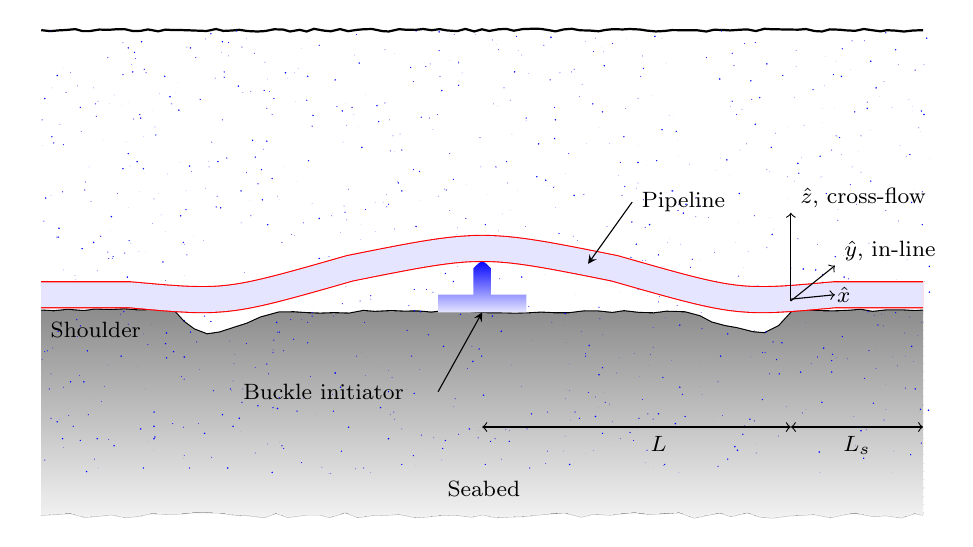
\begin{tikzpicture}[
        scale=0.7,
        annotline/.style = {stealth-},
        arrows1loop/.style={->,red},
        arrows2loop/.style={->,black},
        arrows3loop/.style={->,draw=Gray},
    ]
\pgfmathsetmacro{\aprxglgsize}{16}     

    % Geology
  \draw[thick,smooth, name path=A,decorate, decoration={random steps,amplitude=0.5pt,segment length=3}]  (0.0, 0) to  (\aprxglgsize, 0);
 \draw[thick,smooth, name path=D,decorate, decoration={random steps,amplitude=0.5pt,segment length=5}] (0.0, -.318*\aprxglgsize) -- (0.15*\aprxglgsize, -.318*\aprxglgsize) ..controls (.18*\aprxglgsize,-0.35*\aprxglgsize) .. (.27*\aprxglgsize,-0.32*\aprxglgsize)--(.73*\aprxglgsize,-0.32*\aprxglgsize) ..controls (.82*\aprxglgsize,-0.35*\aprxglgsize) .. (.85*\aprxglgsize,-.318*\aprxglgsize) -- (\aprxglgsize, -.318*\aprxglgsize);
  \draw[thin,smooth, name path=E,decorate, color=gray!50,decoration={random steps,amplitude=1pt,segment length=5}]  (0.0,-.55*\aprxglgsize) to (\aprxglgsize, -.55*\aprxglgsize);
  \tikzfillbetween[ of=D and E, every even segment/.style={bottom color=gray!10, top color = gray!90} ] {pattern=grid};
      \foreach \x in {1,...,1000}
        {
            \pgfmathrandominteger{\a}{1}{1000}
            \pgfmathrandominteger{\b}{1}{500}
            \pgfmathrandominteger{\c}{1}{6}
            \fill[blue] (0.001*\a*\aprxglgsize,-0.001*\b*\aprxglgsize) circle (0.0025*\c);
        };
        %BI
        \shade[top color=blue,bottom color=blue!10]  (.49*\aprxglgsize,-.3*\aprxglgsize) -- (.45*\aprxglgsize,-.3*\aprxglgsize) -- (.45*\aprxglgsize,-.32*\aprxglgsize) -- (.55*\aprxglgsize,-.32*\aprxglgsize) -- (.55*\aprxglgsize,-.3*\aprxglgsize) -- (.51*\aprxglgsize,-.3*\aprxglgsize) -- (.51*\aprxglgsize,-.27*\aprxglgsize) .. controls (.5*\aprxglgsize,-.26*\aprxglgsize) .. (.49*\aprxglgsize,-.27*\aprxglgsize) -- cycle;
    %    \draw[draw=red,double=blue!10,double distance=4pt]  (-4,4) parabola bend (0,0)  (4,4) -- (6,4);
    
        %pipeline
         \draw[draw=red,double=blue!10,double distance=9pt,smooth] (0.0, -.3*\aprxglgsize) -- (0.1*\aprxglgsize, -.3*\aprxglgsize) .. controls (.21*\aprxglgsize,-.31*\aprxglgsize) .. (.35*\aprxglgsize,-.27*\aprxglgsize) .. controls (.5*\aprxglgsize,-.24*\aprxglgsize).. (.65*\aprxglgsize,-.27*\aprxglgsize) .. controls (.79*\aprxglgsize,-.31*\aprxglgsize) ..  (.9*\aprxglgsize,-.3*\aprxglgsize) -- (\aprxglgsize, -.3*\aprxglgsize) ;
  %      \draw[draw=red,double=blue!10,double distance=4pt]  plot [smooth] (0.0, -.3*\aprxglgsize) -- (0.2*\aprxglgsize, -.3*\aprxglgsize) -- (.25*\aprxglgsize,-0.31*\aprxglgsize) -- (.3*\aprxglgsize,-0.32*\aprxglgsize) -- (.35*\aprxglgsize,-0.33*\aprxglgsize) -- (.5*\aprxglgsize,-.34*\aprxglgsize) -- (.65*\aprxglgsize,-0.33*\aprxglgsize) --(.7*\aprxglgsize,-0.32*\aprxglgsize) -- (.75*\aprxglgsize,-0.31*\aprxglgsize) --  (.8*\aprxglgsize,-.3*\aprxglgsize) -- (\aprxglgsize, -.3*\aprxglgsize);
        
%           \draw[draw=red,double=blue!10,double distance=4pt]  plot [smooth] (0.0, -.3*\aprxglgsize) -- (0.2*\aprxglgsize, -.3*\aprxglgsize) -- (.25*\aprxglgsize,-0.31*\aprxglgsize) -- (.3*\aprxglgsize,-0.32*\aprxglgsize) -- (.35*\aprxglgsize,-0.33*\aprxglgsize) -- (.5*\aprxglgsize,-.34*\aprxglgsize) -- (.65*\aprxglgsize,-0.33*\aprxglgsize) --(.7*\aprxglgsize,-0.32*\aprxglgsize) -- (.75*\aprxglgsize,-0.31*\aprxglgsize) --  (.8*\aprxglgsize,-.3*\aprxglgsize) -- (\aprxglgsize, -.3*\aprxglgsize);

 \draw[annotline] (0.62*\aprxglgsize,-0.265*\aprxglgsize) -- ++(0.05*\aprxglgsize,0.07*\aprxglgsize) node[text width=3cm,font=\footnotesize,right] {Pipeline}; 
 \draw[annotline] (0.5*\aprxglgsize,-0.32*\aprxglgsize) -- ++(-0.05*\aprxglgsize,-0.09*\aprxglgsize) node[text width=3cm,font=\footnotesize,left=-0.65cm] {Buckle initiator};         
    \node[text width=2cm,below,font=\footnotesize] at (0.1*\aprxglgsize,-0.32*\aprxglgsize) {Shoulder};
    \node[text width=2cm,below,font=\footnotesize] at (0.55*\aprxglgsize,-0.5*\aprxglgsize) {Seabed};  
    
 %\draw [-stealth](.3*\aprxglgsize, -.28*\aprxglgsize) -- ++(0.05*\aprxglgsize,0.07*\aprxglgsize) {x} ;

\draw[arrows=<-,line width=.4pt](.9*\aprxglgsize, -.3*\aprxglgsize) -- ++(-0.05*\aprxglgsize,-0.005*\aprxglgsize); \path (.91*\aprxglgsize, -.28*\aprxglgsize) node[below,font=\footnotesize] {$\hat{x} $}  ;
\draw[arrows=<-,line width=.4pt](.85*\aprxglgsize, -.207*\aprxglgsize) -- ++(0.0*\aprxglgsize,-0.1*\aprxglgsize); \path (.85*\aprxglgsize, -.19*\aprxglgsize) node[right,font=\footnotesize] {$\hat{z} $, cross-flow}  ;
\draw[arrows=<-,line width=.4pt](.9*\aprxglgsize, -.267*\aprxglgsize) -- ++(-0.05*\aprxglgsize,-0.04*\aprxglgsize); \path (.9*\aprxglgsize, -.25*\aprxglgsize) node[right,font=\footnotesize] {$\hat{y} $, in-line}  ;

%\draw[<->] (.15*\aprxglgsize, -.32*\aprxglgsize) -- (.15*\aprxglgsize, -.375*\aprxglgsize);
%\node[font=\footnotesize] at (.19*\aprxglgsize, -.34*\aprxglgsize) {$s(x)$};


\draw[<->] (.5*\aprxglgsize, -.45*\aprxglgsize) -- ++(.35*\aprxglgsize, 0.*\aprxglgsize); \node[below,font=\footnotesize] at (.7*\aprxglgsize, -.45*\aprxglgsize) {$L$};
\draw[<->] (.85*\aprxglgsize, -.45*\aprxglgsize) -- ++(.15*\aprxglgsize, 0.*\aprxglgsize); \node[below,font=\footnotesize] at (.925*\aprxglgsize, -.45*\aprxglgsize) {$L_s$};

\end{tikzpicture} 
%  \vspace{-20pt} 
  \caption{\label{ISL_system} \footnotesize Schematic of a free-spanning pipeline (not to scale).}
%  \vspace{-20pt} 
\end{figure} 


Since the seabed acts as an elastic foundation, the shoulder-pipeline interaction is described with a stiffness $K_w$ in the vertical direction and a stiffness $K_v$ in the horizontal direction that increase by several orders of magnitude when the material ranges from soft clay to dense sand, as suggested by \cite{Hobbs86}. Since the pipeline can `retain' residual lay tension from its installation history and can experience significant temperature and pressure changes during service, Det Nortske Veritas (\citeyear{DNV-RP-F105,DNV-OS-F101}) recommended that the axial force in the pipeline depends on temperature and pressure. The compressive axial force acting on a given cross section far removed from the ends can be expressed by 
 \begin{equation}\label{axial_force}
 \begin{array}{l } 
\displaystyle  S_e =  (1-2 \nu) \Delta p_i A_i  + E A \alpha_s \Delta T - H_e
  \end{array}  
\end{equation}
where $H_e$ is the effective lay tension, $E$ is Young's modulus, $\nu$ is Poisson's ratio, $\alpha_s$ is the thermal expansion coefficient, $ \Delta p_i $ is the internal pressure difference relative to laying, $A_i$ is the internal cross section of the pipe,  $A$ is the steel cross section of the pipe, and $\Delta T$ is the temperature difference relative to laying. The inertial forces acting on the submerged pipe depend on its effective mass per unit length, $m_e$, expressed by
 \begin{equation}\label{effective_mass}
 \begin{array}{l } 
\displaystyle  m_e = m_s + m_c + m_a
  \end{array}  
\end{equation}
where $m_s$ is the structural mass per unit length, $m_c$ is the mass of the pipe contents (fluid being transported) per unit length, and $m_a$ is the hydrodynamic added mass per unit length calculated based on the outer diameter.  The latter can be expressed as $m_a = c_a \pi \rho_w D^2/4$, where $c_a $ is the added mass coefficient (ranges from 0 to 1.29 according to \cite{Bi:2016aa} and considered as unity in this paper---following \cite{Peek:2021vp}, having the same added mass inside and outside the span is not an important limitation), $\rho_w$ is the seawater density (\SI{1025}{\kilogram\per\meter\cubed}), and $D$ is the outside diameter of the pipe.  
\subsection{Differential equations of motion}
In the appendix (\ref{appendix_first}), the variational problem of beam vibration has been formulated based on Hamilton's principle. 
Considering that the pipeline is suspended when $\hat{x} \le 0$ and in contact with the span shoulder when $\hat{x} > 0$ and using Equation (\ref{system_differential_equation}), the differential equations that govern the motion of the beam can be expressed as follows
 \begin{equation}\label{DiffEqMotion}
 \small
 \begin{array}{l } 
 \text{For the suspended free span section: } -L \le \hat{x} \le 0 \\
\displaystyle  EI \frac{\partial^4 \hat{w}}{\partial \hat{x}^4} + S_e \frac{\partial^2 \hat{w}}{\partial \hat{x}^2}  + m_e \frac{\partial^2 \hat{w}}{\partial \hat{t}^2} = \frac{EA}{2(L+L_s)} \frac{\partial^2 \hat{w}}{\partial \hat{x}^2} \int_{-L}^0 \left\{\left( \frac{\partial \hat{v}}{\partial \hat{x}}  \right)^2 +  \left(\frac{\partial \hat{w}}{\partial \hat{x}}  \right)^2 \right\} d\hat{x} + \hat{q} (\hat{x},\hat{t}) \\
\text{and for pipeline on shoulder: }\hat{x} > 0 \\
\displaystyle  EI \frac{\partial^4 \hat{w}}{\partial \hat{x}^4} + S_e \frac{\partial^2 \hat{w}}{\partial \hat{x}^2} + m_e \frac{\partial^2 \hat{w}}{\partial \hat{t}^2} + K_w \hat{w}  =  \hat{q} (\hat{x},\hat{t})  
  \end{array}  
\end{equation}
where $\hat{w} (\hat{x},\hat{t})$ is the deflection at position $\hat{x}$ and time $\hat{t}$. We refer to $\hat{w}$ as the displacement in the transversal direction and it can be horizontal (in-line) or vertical (cross-flow) depending on the nature of $\hat{q} (\hat{x},\hat{t})$. The displacement $\hat{v}$ is the lateral deflection, $I$ is the second moment of area, $\hat{q}$ is due to drag and inertia hydrodynamic forces (if the problem is in-line) or due to self-weight and lift hydrodynamic forces (if the problem is cross-flow), and $K_w $ is the soil stiffness. In Equation (\ref{DiffEqMotion}), the terms $\left( \frac{\partial \hat{v}}{\partial \hat{x}}  \right)^2$ and $\left(\frac{\partial \hat{w}}{\partial \hat{x}}  \right)^2$ represent mid-plane stretching in the lateral and transversal directions, respectively. They are assumed to act on the suspended free span section only (they are negligible on the shoulder for simplification). 

It is convenient to use the following non-dimensional variables 
 \begin{equation}\label{NonDimensionalVar}
 \begin{array}{l } 
\displaystyle   x = \frac{\hat{x}}{L}; \quad  v = \frac{\hat{v}}{r}; \quad  w = \frac{\hat{w}}{r}; \quad  t = \hat{t} \sqrt{\frac{EI}{m_e L^4}} ; \quad \text{ and }  \Omega = \omega\sqrt{ \frac{m_e L^4}{EI}}
  \end{array}  
\end{equation}
where $r = \sqrt{I/A}$ is the cross section's radius of gyration and $\omega$ is a frequency of vibration. Therefore, Equation (\ref{DiffEqMotion}) can be rewritten 

 \begin{equation}\label{DiffEqMotion_nondim}
 \begin{array}{l } 
\displaystyle  \frac{\partial^4 w}{\partial x^4} + S \frac{\partial^2 w}{\partial x^2}  + \frac{\partial^2 w}{\partial t^2} = \frac{\iota}{2} \frac{\partial^2 w}{\partial x^2} \int_{-1}^0 \left\{\left( \frac{\partial v}{\partial x}  \right)^2 + \left(  \frac{\partial w}{\partial x}  \right)^2 \right\}dx+ q (x,t) \text{ for } -1 \le x \le 0 \\
\displaystyle  \frac{\partial^4 w}{\partial x^4} + S \frac{\partial^2 w}{\partial x^2} + \frac{\partial^2 w}{\partial t^2} + \kappa^4 w  =  q (x,t) \text{ for } x > 0
  \end{array}  
\end{equation}
where 
 \begin{equation}\label{NonDimensionalquantities}
 \begin{array}{l } 
\displaystyle   S = \frac{S_e L^2}{EI}; \quad \iota = \frac{L}{L+L_s}; \quad  q = \frac{\hat{q} L^4}{rEI}; \quad \text{ and }  \kappa^4 = \frac{K_w L^4}{EI}
  \end{array}  
\end{equation}
are non-dimensional quantities representing the axial force, span ratio, distributed transversal force, and seabed stiffness, respectively. For a given solution to the problem, the effect of mid-plane stretching in the lateral and transversal directions can be included in the variable \[ \Lambda = \frac{\iota}{2} \int_{-1}^0  \left\{\left( \frac{\partial v}{\partial x}  \right)^2 + \left(  \frac{\partial w}{\partial x}  \right)^2 \right\} dx \] Hence, Equation (\ref{DiffEqMotion_nondim}) can be expressed as follows:
%For simplification, we assume that $\int_{-1}^0 \left( \frac{\partial w}{\partial x}  \right)^2 dx  \approx \left( \frac{\delta}{r}  \right)^2 $ where $\delta$ is the maximum deflection at the buckle initiator. Hence, Equation {DiffEqMotion_nondim} can be expressed as follows:

 %\begin{equation}\label{DiffEqMotionNewNondim}
% \begin{array}{l } 
%\displaystyle  \frac{\partial^4 w}{\partial x^4} + \lambda^2_{\delta} \frac{\partial^2 w}{\partial x^2}  + \frac{\partial^2 w}{\partial t^2} = q (x) \text{ for } -1 \le x \le 0 \\
%\displaystyle  \frac{\partial^4 w}{\partial x^4} + \lambda^2_0 \frac{\partial^2 w}{\partial x^2} + \frac{\partial^2 w}{\partial t^2} + K w  =  q (x) \text{ for } x > 0
%  \end{array}  
%\end{equation}
%where $\lambda^2_{\delta} = S- \frac{1}{2}\left( \frac{\delta}{r}  \right)^2$ is a constant that represents the non-dimensional critical buckling load. 

 \begin{equation}\label{DiffEqMotionNewNondim}
 \begin{array}{l } 
\displaystyle  \frac{\partial^4 w}{\partial x^4} + \eta ^2 \frac{\partial^2 w}{\partial x^2}  + \frac{\partial^2 w}{\partial t^2} = q (x,t) \text{ for } -1 \le x \le 0 \\
\displaystyle  \frac{\partial^4 w}{\partial x^4} + S \frac{\partial^2 w}{\partial x^2} + \frac{\partial^2 w}{\partial t^2} + \kappa^4 w  =  q (x,t) \text{ for } x > 0
  \end{array}  
\end{equation}
where $\eta^2 = S-\Lambda$ is a constant that represents the non-dimensional axial load. Solving Equation (\ref{DiffEqMotionNewNondim}) requires the definition of initial conditions (e.g. the original boundary displacement of the pipeline at rest) and the definition of boundary conditions, which can be idealised (fixed-fixed, pinned-pinned etc.) or made more realistic (interaction with the seabed).  

\subsection{Model verification}
Before detailing the solution method under various conditions of loading in the subsequent sections, it is worthwhile to compare the results of the proposed model with those from finite element modelling. The general-purpose finite element software package Abaqus was used to create the finite element model. A solid beam with a circular cross-section, diameter $D =$ \SI{45.2}{\centi\meter}, span length $L = 75D$, shoulder length $L_s = L$, and buckle initiator height $\hat{H} = 1.33 D$  was developed for simulation (see Figure \ref{ISL_system}). The spanning area was horizontally deviated by a slope of $D/L$ to simulate the lateral mid-plane stretching. The beam was made of steel with density $\rho =$ \SI{7800}{\kilogram\per\meter\cubed} and elastic modulus $E =$ \SI{200}{\giga\pascal}. An elastic foundation with stiffness $K_w = 100 kN/m/m$ was used to simulate the shoulder. The numerical simulation consisted of a non-linear quasistatic loading step to attain geostatic equilibrium followed by modal analysis to calculate the modes and frequencies of vibration. During these steps, the beam was subjected to gravity but constrained from moving at the buckle initiator, and allowed to move vertically at the extreme point of the shoulder. Under these loading conditions, Figure \ref{ModelVerification}-a shows the static deflection of the beam obtained using the proposed model and the finite element method. In addition, Figure \ref{ModelVerification}-b shows the natural frequencies obtained for different modes of vibration and elastic elastic foundation stiffnesses. Figure \ref{ModelVerification} demonstrates the excellent agreement between the proposed model and the finite element method, which gives confidence in the predictive ability of the proposed method. 

\begin{figure}[H]
\begin{center}
\begin{tabular}{c c}
\begin{tikzpicture}
\node (image) at (0,0) { 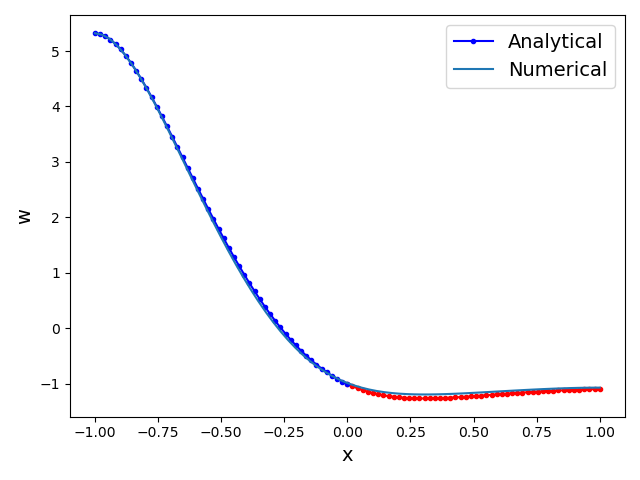
\includegraphics[width=0.5\hsize]{Verification_W_X.png}};
%\node[circle,white,fill=black] at (-2,2){\small (a)};
\node[left,black,fill=white]at (0.5,3.25) {\small (a)};
\end{tikzpicture}
 & 
 \begin{tikzpicture}
\node (image) at (0,0) { 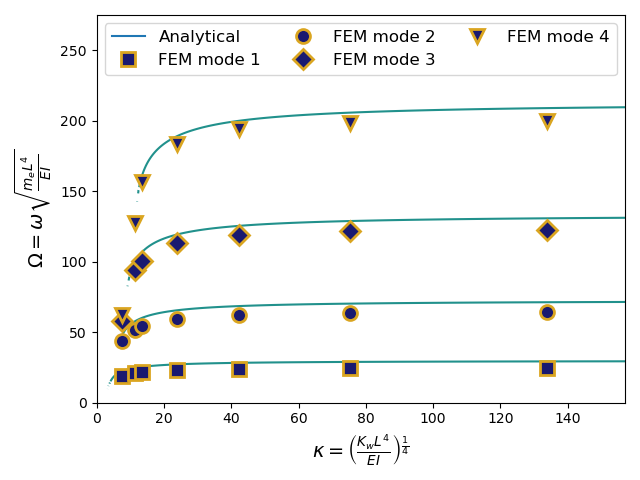
\includegraphics[width=0.5\hsize]{Verification_Omg_K.png}};
%\node[circle,white,fill=black] at (-2,2){\small (a)};
\node[left,black,fill=white]at (0.5,3.25) {\small (b)};
\end{tikzpicture}  
\end{tabular}
 \caption{\label{ModelVerification} Verification of the proposed model using the finite element method. }
\end{center}
\end{figure}


\section{Static response with lateral mid-plane stretching}
The deformed shape of the pipeline, including the sag geometry, can be obtained by solving the quasi-static version of Equation (\ref{DiffEqMotionNewNondim}) given specific boundary conditions. In this section, we take into account the lateral mid-plane stretching and ignore the transversal mid-plane stretching for simplification; the latter will be considered in Section \ref{Dynamic_Response}. The deformed shape depends on the initial geometry, stiffness of the pipe, interaction with the seabed, effects of gravity and hydrodynamic forces, and history of loading. For example, high tensions in the pipe and/or stiff shoulders reduce the pipe deflection into the span. Assuming that $q(x)$ is uniform, ignoring the term $\frac{\partial^2 w}{\partial t^2}$ in Equation (\ref{DiffEqMotionNewNondim}), and solving these differential equations results in the following expressions 
\begin{equation}\label{StaticSolution}
 \begin{array}{l } 
\displaystyle   w^-(x)=  \frac{q x^2}{2 \eta^2} + A_1 + A_2 x + A_3 \cos \eta x  + A_4 \sin \eta  x; \quad  \text{ for } -1 \le x \le 0 \\
\displaystyle   w^+(x)=  \frac{q }{k} + \left(A_5 \cos \alpha_2 x +  A_6 \sin \alpha_2 x\right)e^{-\alpha_1 x}   +  \left(A_7 \cos \alpha_2 x +  A_8 \sin \alpha_2 x\right)e^{\alpha_1 x} ; \text{ for } x > 0
  \end{array}  
\end{equation}
where $\alpha_1 = \sqrt{\frac{\kappa^2}{2} - \frac{S}{4}}$, $\alpha_2 = \sqrt{\frac{\kappa^2}{2} + \frac{S}{4}}$, $w(x) =w^-(x)$ within the suspended portion of the pipeline and $w(x) =w^+(x)$ on the laid portion interacting with the shoulder. The expression of displacement on elastic foundation, $w^+(x)$, is valid provided that $\eta_0^2 \le 2 \kappa^2$.  For the displacement to remain finite on a long shoulder, the term $\left(A_7 \cos \alpha_2 x +  A_8 \sin \alpha_2 x\right)e^{\alpha_1 x}$ has to vanish. Matching the displacements and their space derivatives at the interface $w$, $w'$, $w''$, and $w'''$ yields the following relations: 

\begin{equation}\label{Continuity}
 \begin{array}{l } 
\displaystyle   A_1 + A_3 = \frac{q}{k}  + A_5\\
\displaystyle   A_2 + \eta A_4 = -\alpha_1 A_5 + \alpha_2 A_6 \\
\displaystyle   \frac{q}{\eta^2} - \eta^2 A_3 = (\alpha_1^2 - \alpha_2^2) A_5 - 2 \alpha_1 \alpha_2 A_6 \\
\displaystyle   \eta^3 A_4 = \alpha_1 (\alpha_1^2 - 3 \alpha_2^2) A_5 + \alpha_2 (\alpha_2^2 - 3 \alpha_1^2) A_6 \\
  \end{array}  
\end{equation}

Given the symmetry of the pipeline at the point of contact with the buckle initiator (see Figure \ref{ISL_system}), it is possible to consider that the displacement has a flat tangent ($w'(-1) =  0$). In addition, it is convenient to assume that the displacement $\hat{w}(-L) =  \hat{H}$ (or its non-dimensional equivalent  $w(-1) =  -H$). Therefore, two additional equations can be obtained to close the system:

\begin{equation}\label{BoundaryConditions_01}
 \begin{array}{l } 
\displaystyle   \frac{q}{2 \eta^2} + A_1 -A_2 + \cos \eta A_3 -  \sin \eta A_4 = -H \\
\displaystyle   - \frac{q}{\eta^2} + A_2 + \eta  \sin \eta A_3 + \eta  \cos \eta A_3 = 0 \\ 
  \end{array}  
\end{equation} 

The linear system of equations (\ref{Continuity}) and (\ref{BoundaryConditions_01}) can be solved to obtain the coefficients $(A_i)_{i=1..6}$. The closed form solution also requires the calculation of $\displaystyle \Lambda = \frac{\iota}{2} \int_{-1}^0  \left\{\left( \frac{\partial v}{\partial x}  \right)^2 \right\} dx $ given that the lateral mid-plane stretching is considered and the transversal mid-plane stretching is ignored. We assume that $v$ is independent of time and that the profile of lateral deflection is known, which means that $\Lambda$ is an input parameter. For the particular case $L_s=L$ and $\frac{\partial v}{\partial x} = \frac{D}{r}$, we deduce $\iota = \frac{1}{2}$ and  $\Lambda =  \left(\frac{D}{r}\right)^2$. With the coefficients $(A_i)_{i=1..6}$ and the constant $\Lambda$ at hand, the solution (\ref{StaticSolution}) of the static problem is determined. 

Figure \ref{EffectsOfImprfections} shows the results obtained for the following parameters unless specified otherwise: $D =$ \SI{45.2}{\centi\meter}, wall thickness $D/15$, original span length $L = 75D$, pipe averaged density $\rho =$ \SI{2200}{\kilogram\per\meter\cubed}, elastic modulus $E =$ \SI{200}{\giga\pascal}, soil stiffness $K_w = 100 kN/m/m$, thermal expansion coefficient $\alpha_s =$ \SI{ 1d-5}{\per\celsius}, and temperature change $\Delta T =$ \SI{40}{\celsius}.




\begin{figure}[hbtp]
\begin{center}
\begin{tabular}{c c}
\begin{tikzpicture}
\node (image) at (0,0) { 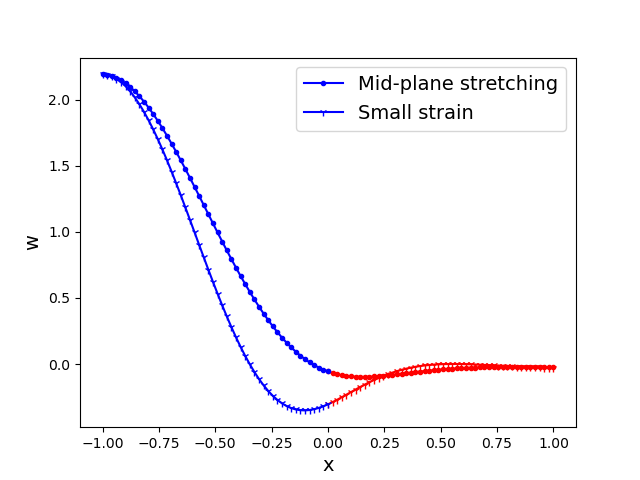
\includegraphics[width=0.5\hsize]{effect_of_stretching.png}};
%\node[circle,white,fill=black] at (-2,2){\small (a)};
\node[left,black,fill=white]at (0,2.75) {\small (a)};
\end{tikzpicture}
 & 
 \begin{tikzpicture}
\node (image) at (0,0) { 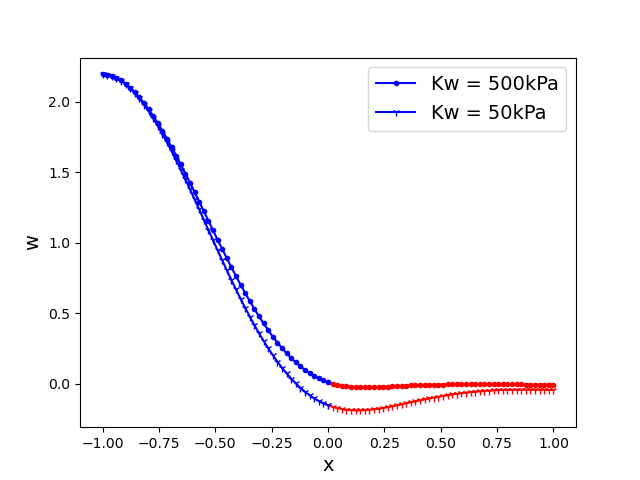
\includegraphics[width=0.5\hsize]{effect_soil_stiffness.png}};
%\node[circle,white,fill=black] at (-2,2){\small (a)};
\node[left,black,fill=white]at (0,2.75) {\small (b)};
\end{tikzpicture}
\\
%\begin{tikzpicture}
%\node (image) at (0,0) { \includegraphics[width=0.5\hsize]{effect_Axial_Force.png}};
%%\node[circle,white,fill=black] at (-2,2){\small (a)};
%\node[left,black,fill=white]at (0,1.8) {\small (c)};
%\end{tikzpicture}
% & 
% \begin{tikzpicture}
%\node (image) at (0,0) { \includegraphics[width=0.5\hsize]{effect_of_distributed_force.png}};
%%\node[circle,white,fill=black] at (-2,2){\small (a)};
%\node[left,black,fill=white]at (0,1.8) {\small (d)};
%\end{tikzpicture}  
%\\
\begin{tikzpicture}
\node (image) at (0,0) { 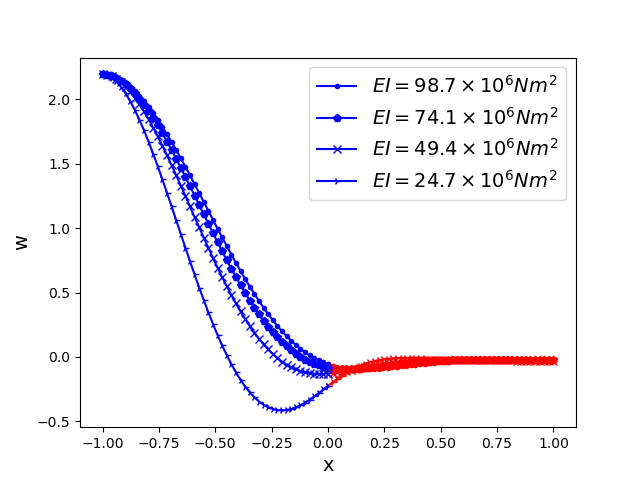
\includegraphics[width=0.5\hsize]{effect_of_flexural_stiffness.png}};
%\node[circle,white,fill=black] at (-2,2){\small (a)};
\node[left,black,fill=white]at (0,2.75) {\small (c)};
\end{tikzpicture}
 & 
 \begin{tikzpicture}
\node (image) at (0,0) { 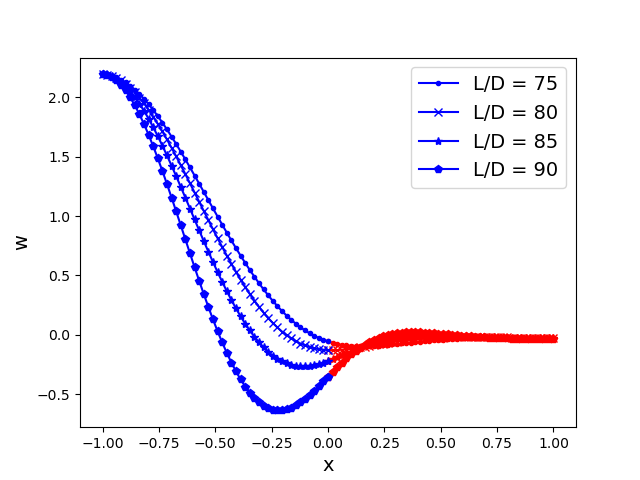
\includegraphics[width=0.5\hsize]{effect_of_length.png}};
%\node[circle,white,fill=black] at (-2,2){\small (a)};
\node[left,black,fill=white]at (0,2.75) {\small (d)};
\end{tikzpicture}
\end{tabular}
 \caption{\label{EffectsOfImprfections} Response of a free spanning partially supported pipeline under the effects of (a) mid-plane stretching, (b) soil stiffness, (c) flexural stiffness, and (d) span length. }
\end{center}
\end{figure}

\section{Eigenvalue problem of the pipeline with lateral mid-plane stretching} 
In the context of free spanning pipelines subjected to VIV, the eigenvalue problem is solved to evaluate the eigenfrequencies and modeshapes due to flow-induced vibration, which then enables the calculation of fatigue damage---a step that is omitted in this study. In-line and cross-flow vibrations are either treated independently or dealt with in an integrated manner. When the principle of superposition is valid (i.e. in the linear regime), the modeshapes are combined linearly to estimate the response of the structure to time-depending loading conditions such as VIV. The magnitude of the response depends on the closeness of vortex shedding frequency to one of the natural frequencies of the pipeline. 

When the frequency of vortex shedding is significantly far from its natural frequencies, the impact of vortex shedding is minimal and the dynamic deflections of the pipe are not significant compared to the static deflection. However, as the frequency of vortex shedding approaches one of the natural frequencies, the amplitude of the forced vibration increases tremendously and produces resonance. In the absence of damping, the amplitudes of vibration can be high enough to cause concrete spilling (if the pipeline is coated or lined with concrete) and other structural failures. Therefore, it is sensible to establish a safety buffer between the natural frequencies of the pipe and the vortex shedding frequency to avoid failure due to resonance. To calculate the natural frequencies of the system at hand, we solve the eigenvalue problem by linearising the dynamic response of the pipeline around its static response and assuming a harmonic response with respect to time. To this end, the displacement is expressed by 
 \begin{equation}\label{splittedDisplacement}
 \begin{array}{l }  
 w(x,t) = \phi_0(x) + \phi(x)e^{-i\Omega t}
  \end{array}  
\end{equation}
where $\phi_0$ is the static component and $\phi(x)e^{-i\Omega t}$ is the dynamic component of the response. Hence, the differential equations (\ref{DiffEqMotion_nondim}) governing the system can be written as follows
 \begin{equation}\label{DiffEqMotion_nondim_dynamics}
 \begin{array}{l } 
\displaystyle  \frac{\partial^4 \phi}{\partial x^4} + \eta^2 \frac{\partial^2 \phi}{\partial x^2}  - \Omega^2 \phi  =  0  \text{ for } -1 \le x \le 0 \\
\displaystyle  \frac{\partial^4 \phi}{\partial x^4} + S \frac{\partial^2 \phi}{\partial x^2}   + (\kappa^4- \Omega^2) \phi  = 0 \text{ for } x > 0
  \end{array}  
\end{equation}
where $\eta^2 = S-\Lambda$ and $\displaystyle \Lambda = \frac{\iota}{2} \int_{-1}^0  \left\{\left( \frac{\partial v}{\partial x}  \right)^2 \right\} dx $ in the presence of lateral mid-plane stretching and absence of transversal mid-plane stretching. 

\subsection{Dynamics of free spanning pipeline with quasi-static shoulder and axial force}
As a first case, assume that the side of the pipeline that is supported by the span shoulder is quasi-static. This means $\phi (x)$ and $\phi' (x) = 0$ $\forall x > 0$. Hence, the eigenvalue problem of interest is  
 \begin{equation}\label{DiffEqMotion_nondim_dynamics}
 \begin{array}{l } 
\displaystyle  \frac{\partial^4 \phi}{\partial x^4} + 2P \frac{\partial^2 \phi}{\partial x^2}  - \Omega^2 \phi  =  0  \text{ for } -1 \le x \le 0 \\ 
\displaystyle \phi (-1) = \phi (0) =0 \text{ and }  \phi' (-1) = \phi' (0) =0 
  \end{array}  
\end{equation}
where $2P = \eta^2 = S-\Lambda$ to simplify the notations. The solution of Equation (\ref{DiffEqMotion_nondim_dynamics}) reads: 
 \begin{equation}\label{SolutionDiffEqMotion_nondim_dynamics}
 \begin{array}{l } 
\displaystyle  \phi(x) = B_1 \cosh \gamma_1 x + B_2 \sinh \gamma_1 x + B_3 \cos \gamma_2 x + B_4 \sin \gamma_2 x \\
\displaystyle \phi (-1) = \phi' (-1) =0 \text{ and }  \phi (0) = \phi' (0) =0 
  \end{array}  
\end{equation}
where $\gamma_1 = \sqrt{\sqrt{P^2 + \Omega^2}-P}$ and $ \gamma_2 = \sqrt{\sqrt{P^2 + \Omega^2}+P}$. Implementing the boundary conditions shown in Equation (\ref{SolutionDiffEqMotion_nondim_dynamics}) results in the following system of equations 
 \begin{equation}\label{NonTrivialSolution}
 \begin{array}{l } 
\displaystyle  B_1 +  B_3 =0; \quad  \gamma_1 B_2 +  \gamma_2 B_4 =0 \\
\displaystyle \cosh \gamma_1 B_1   -  \sinh \gamma_1 B_2 +  \cos \gamma_2 B_3  - \sin \gamma_2 B_4 =0   \\
\displaystyle  \gamma_1  \sinh \gamma_1 B_1 - \gamma_1 \cosh \gamma_1 B_2  - \gamma_2  \sin \gamma_2 B_3  - \gamma_2  \cos \gamma_2 B_4 =0  \\
  \end{array}  
\end{equation}
The non-trivial solution of this set of equations can be obtained by setting its determinantal equation to zero, which results in the following characteristic equation:
 \begin{equation}\label{NonTrivialSolution-1}
 \begin{array}{l } 
\displaystyle  2\gamma_1\gamma_2\left(1-\cosh \gamma_1 \cos \gamma_2\right)+\left(\gamma_1^2-\gamma_2^2\right)\sinh \gamma_1 \sin \gamma_2 = 0
  \end{array}  
\end{equation}

Equation (\ref{NonTrivialSolution-1}) is equivalent to the characteristic equations derived by \cite{Bokaian:1990tk} and \cite{Liu1996VibrationOA}. It has no explicit analytical solution but can be analysed numerically as shown in Figure (\ref{Frequencies_analysis}) indicating the variation of non-dimensional frequency $\Omega$ with respect to axial forces and the seabed stiffness. Figure (\ref{Frequencies_analysis}-a) shows the effect of non-dimensional axial force on the non-dimensional frequency in the case of a spanning pipeline with a quasi-static shoulder obtained by solving Equation (\ref{DiffEqMotion_nondim_dynamics}). This figure also shows that the non-dimensional frequency reduces when the axial force increases and increases when mid-plane stretching is accounted for. 
  
 
 \begin{figure}[hbtp]
\begin{center}
\begin{tabular}{c c}
\begin{tikzpicture}
%left bottom right top
\node (image) at (0,0) {\adjincludegraphics[valign=M,trim={0 0 0 0},clip,width=0.5\hsize]{ClampedClampedFreqOM_P.png}};
%\node[circle,white,fill=black] at (-2,2){\small (a)};
\node[left,black,fill=white]at (0.5,3.25) {\small (a)};
\end{tikzpicture}
 & 
 \begin{tikzpicture}
\node (image) at (0,0) { \adjincludegraphics[valign=M,trim={0 0 0 0},clip,width=0.5\hsize]{ClampedShoulderFreqOM_K.png}};
%\node[circle,white,fill=black] at (-2,2){\small (a)};
\node[left,black,fill=white]at (0.5,3.25) {\small (b)};
\end{tikzpicture} \\
\begin{tikzpicture}
\node (image) at (0,0) {\adjincludegraphics[valign=M,trim={0 0 0 0},clip,width=0.5\hsize]{ClampedShoulderwithForceFreqOM_P.png}};
%\node[circle,white,fill=black] at (-2,2){\small (a)};
\node[left,black,fill=white]at (0.5,3.25) {\small (c)};
\end{tikzpicture}
 & 
 \begin{tikzpicture}
\node (image) at (0,0) { \adjincludegraphics[valign=M,trim={0 0 0 0},clip,width=0.5\hsize]{ClampedShoulderwithForceFreqOM_K.png}};
%\node[circle,white,fill=black] at (-2,2){\small (a)};
\node[left,black,fill=white]at (0.5,3.25) {\small (d)};
\end{tikzpicture} 
\end{tabular}
 \caption{\label{Frequencies_analysis} Variation of non-dimensional frequency $\Omega$ with (a) non-dimensional axial force for a spanning pipeline with quasi-static shoulder (b) non-dimensional shoulder stiffness for a dynamic spanning and shoulder-supported pipeline without axial force, (c) non-dimensional axial force for a dynamic spanning and shoulder-supported pipeline with axial force (results obtained at $\kappa = 20$), and (d) non-dimensional shoulder stiffness for a dynamic spanning and shoulder-supported pipeline with axial force (results obtained at $S = 20$).  }
\end{center}
\end{figure}

\subsection{Dynamics of free spanning pipeline with vibrating shoulder and without axial force}
This case assumes that vibration occurs both in the spanning and shoulder-supported zones of the pipeline. Based on Equation (\ref{DiffEqMotion_nondim_dynamics}), the system of differential equations that governs the pipeline can be used to derive the following eigenvalue problem:  
 \begin{equation}\label{DiffEqMotion_nondim_dynamics_1}
 \begin{array}{l } 
\displaystyle  \frac{\partial^4 \phi}{\partial x^4} + 2P  \frac{\partial^2 \phi}{\partial x^2}  - \Omega^2 \phi  =  0  \text{ for } -1 \le x \le 0 \\
\displaystyle  \frac{\partial^4 \phi}{\partial x^4}   + (\kappa^4- \Omega^2) \phi  = 0 \text{ for } x > 0
  \end{array}  
\end{equation}
where $2P = -\Lambda$. The solution of Equation (\ref{DiffEqMotion_nondim_dynamics_1}) reads 
 \begin{equation}\label{SolutionDiffEqMotion_nondim_dynamics_1}
 \begin{array}{l } 
\displaystyle  \phi (x)= C_1 \cosh \gamma_1 x + C_2 \sinh \gamma_1 x + C_3 \cos \gamma_2 x + C_4 \sin \gamma_2 x  \text{ for } -1 \le x \le 0 \\
\displaystyle  \phi (x)= e^{-\zeta x}  \left(C_5 \cos \zeta x +  C_6 \sin \zeta x\right)  + e^{\zeta x}  \left(C_7 \cos \zeta x +  C_8 \sin \zeta x\right); \text{ for } x > 0
  \end{array}  
\end{equation}
where $\zeta = \left(\frac{\kappa^4 - \Omega^2}{4}\right)^{\frac{1}{4}}$, $\phi(x) =\phi^-(x)$ within the suspended portion of the pipeline and $\phi(x) =\phi^+(x)$ on the laid portion interacting with the shoulder. For the displacement to remain finite on a long shoulder, the term $ \left(C_7 \cos \zeta x +  C_8 \sin \zeta x\right)e^{\zeta x}$ has to vanish. Proceeding like for the static solution (\ref{StaticSolution}) and matching the displacements and their space derivatives at the interface $\phi$, $\phi'$, $\phi''$, and $\phi'''$ yields the following relations: 

\begin{equation}\label{Continuity_1}
 \begin{array}{l } 
\displaystyle   C_1 + C_3 = C_5\\
\displaystyle  \gamma_1 C_2 + \gamma_2 C_4 = -\zeta C_5 + \zeta C_6 \\
\displaystyle  \gamma_1^2 C_1 - \gamma_2^2 C_3 = -2 \zeta^2 C_6 \\
\displaystyle  \gamma_1^3 C_2 - \gamma_2^3 C_4 = 2\zeta^3 C_5 + 2\zeta^3 C_6 \\
  \end{array}  
\end{equation}

Given the symmetry of the pipeline at the buckle initiator, it is possible to consider that $ \phi (-1) = \phi' (-1) =0$. Therefore, two additional equations can be obtained to close the system:

\begin{equation}\label{BoundaryConditions}
 \begin{array}{l }   
\displaystyle    \cosh \gamma_1 C_1 - \sinh \gamma_1 C_2 + \cos \gamma_2C_3   -  \sin \gamma_2 C_4= 0 \\
\displaystyle   \gamma_1 \sinh \gamma_1 C_1 - \gamma_1 \cosh \gamma_1 C_2 -  \gamma_2 \sin  \gamma_2C_3   -   \gamma_2 \cos \gamma_2 C_4 = 0 \\
  \end{array}  
\end{equation} 

The non-trivial solution of this set of equations can be obtained by calculating the zero of the characteristic equation. Figure (\ref{Frequencies_analysis}-b) shows the variation of non-dimensional frequency $\Omega$ with respect to non-dimensional shoulder stiffness for a dynamic spanning and shoulder-supported pipeline without axial force. This result was obtained by solving Equation (\ref{DiffEqMotion_nondim_dynamics_1}). It can be seen that the non-dimensional frequency increases non-linearly with the seabed shoulder stiffness. In addition, the figure indicates that the frequency increases when the mid-plane stretching is considered. 

\subsection{Dynamics of free spanning pipeline with vibrating shoulder and axial force}
The present scenario exhibits similarities with the previous case in terms of vibration occurring in both the spanning and shoulder-supported areas of the pipeline. However, there is a notable difference as this scenario takes into account the axial force. Based on Equation (\ref{DiffEqMotion_nondim_dynamics}), the eigenvalue problem that describes the pipeline under axial force can be written as follows:  
 \begin{equation}\label{DiffEqMotion_nondim_dynamics_2}
 \begin{array}{l } 
\displaystyle  \frac{\partial^4 \phi}{\partial x^4} + 2P  \frac{\partial^2 \phi}{\partial x^2}  - \Omega^2 \phi  =  0  \text{ for } -1 \le x \le 0 \\
\displaystyle  \frac{\partial^4 \phi}{\partial x^4}   + S  \frac{\partial^2 \phi}{\partial x^2} - (\kappa^4- \Omega^2) \phi  = 0 \text{ for } x > 0
  \end{array}  
\end{equation}
where $2P = S -\Lambda$. The solution of Equation (\ref{DiffEqMotion_nondim_dynamics_2}) reads 
 \begin{equation}\label{SolutionDiffEqMotion_nondim_dynamics_2}
 \begin{array}{l } 
\displaystyle  \phi (x)= D_1 \cosh \gamma_1 x + D_2 \sinh \gamma_1 x + D_3 \cos \gamma_2 x + D_4 \sin \gamma_2 x  \text{ for } -1 \le x \le 0 \\
\displaystyle  \phi (x)=  e^{-\zeta_1 x} \left(D_5 \cos \zeta_2 x +  C_6 \sin \zeta_2 x\right)  +  e^{-\zeta_1 x} \left(C_7 \cos \zeta_2 x +  C_8 \sin \zeta_2 x\right) ; \text{ for } x > 0
  \end{array}  
\end{equation}
where $\zeta_1 = \sqrt{\sqrt{\frac{\kappa^4 - \Omega^2}{4}} - \frac{S}{4}}$ and $\zeta_2 = \sqrt{\sqrt{\frac{\kappa^4 - \Omega^2}{4}} + \frac{S}{4}}$. 

As for the previous cases, the term $ \left(D_7 \cos \zeta_1 x +  D_8 \sin \zeta_1 x\right)e^{\zeta_2 x}$ has to vanish so that the displacement remains finite. Matching the displacements and their space derivatives at the interface and applying the boundary conditions at the pipeline at the buckle initiator (i.e. $ \phi (-1) = \phi' (-1) =0$) results in: 

\begin{equation}\label{Continuity_2}
 \begin{array}{l } 
\displaystyle   D_1 + D_3 = D_5\\
\displaystyle  \gamma_1 D_2 + \gamma_2 D_4 = -\zeta_1 D_5 + \zeta_2 D_6 \\
\displaystyle  \gamma_1^2 D_1 - \gamma_2^2 D_3 = (\zeta_1^2 -\zeta_2^2)D_5 -2 \zeta_1\zeta_2 C_6 \\
\displaystyle  \gamma_1^3 D_2 - \gamma_2^3 D_4 = - \zeta_1 (\zeta_1^2 - 3\zeta_2^2) D_5 - \zeta_2 (\zeta_2^2 - 3\zeta_1^2) D_6 \\
\displaystyle    \cosh \gamma_1 D_1 - \sinh \gamma_1 D_2 + \cos \gamma_2D_3   -  \sin \gamma_2 D_4= 0 \\
\displaystyle   \gamma_1 \sinh \gamma_1 D_1 - \gamma_1 \cosh \gamma_1 D_2 -  \gamma_2 \sin  \gamma_2D_3   -   \gamma_2 \cos \gamma_2 D_4 = 0 \\
  \end{array}  
\end{equation}

Setting the characteristic equation of the system (\ref{Continuity_2}) to zero results in a non-trivial solution in terms of natural frequencies. Figure (\ref{Frequencies_analysis}-c) shows the variation of non-dimensional frequency $\Omega$ with respect non-dimensional axial force for a free spanning and shoulder-supported pipeline with axial force (results obtained at $\kappa = 20$). This figure also shows that the non-dimensional frequency reduces when the axial force increases and increases when mid-plane stretching is taken into consideration. Comparing Figures (\ref{Frequencies_analysis}-a) and (\ref{Frequencies_analysis}-c) shows that the non-dimensional frequency $\Omega$ is generally lower when the dynamic response of the shoulder-supported pipeline is considered.


Similarly, Figure (\ref{Frequencies_analysis}-d) shows the variation of non-dimensional frequency $\Omega$ with respect non-dimensional shoulder stiffness for a dynamic spanning and shoulder-supported pipeline with axial force (results obtained at $S = 20$). Comparing Figures (\ref{Frequencies_analysis}-b) and (\ref{Frequencies_analysis}-d) indicates that the non-dimensional frequency increases non-linearly with seabed shoulder stiffness and that the frequency increases when the mid-plane stretching is considered. However, the two figures show that the frequency reduces when the axial force is increased. 


\subsection{Effective length}
The effective length of a pipeline having an actual span $L$ is the length $L_e$ that would have been obtained if the pipeline were to buckle as a pinned-pinned column. Ideal boundary conditions such as pin-pin and fixed-fixed result in $\frac{L_e}{L}$ ratios of 1 and 0.664, respectively. Based on the analysis of \cite{Hobbs86}, we can calculate it using the ratio \[\frac{L_e}{L} = \frac{\pi}{\sqrt{\Omega}}\] Figure \ref{Effective_length_Analysis} shows the variation of effective length with the non-dimensional shoulder stiffness. The results indicate that low seabed stiffness results in effective lengths that are closer to span length, which is closer to the ideal pin-pin condition. However, high seabed stiffness pushes the effective length to a fraction of span length that makes is closer to an ideal fixed-fixed condition. More importantly, the effective length is lower when the mid-plane stretching is taken into account. 


 \begin{figure}[hbtp]
\begin{center}
\begin{tabular}{c c}
\begin{tikzpicture}
\node (image) at (0,0) { 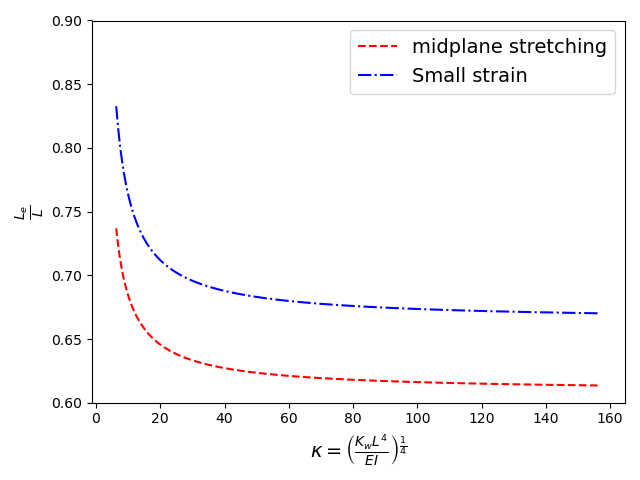
\includegraphics[width=0.5\hsize]{ClampedShoulder_effectivelength.png}};
%\node[circle,white,fill=black] at (-2,2){\small (a)};
\node[left,black,fill=white]at (0.5,3.25) {\small (a)};
\end{tikzpicture}
 & 
 \begin{tikzpicture}
\node (image) at (0,0) { 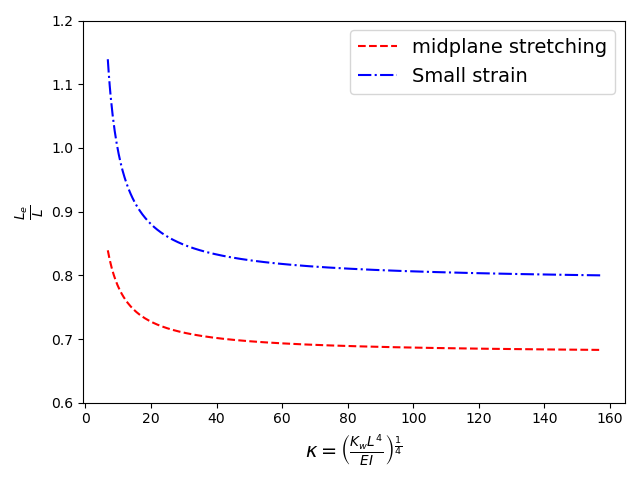
\includegraphics[width=0.5\hsize]{ClampedShoulderWithForce_effectivelength.png}};
%\node[circle,white,fill=black] at (-2,2){\small (a)};
\node[left,black,fill=white]at (0.5,3.25) {\small (b)};
\end{tikzpicture}  
\end{tabular}
 \caption{\label{Effective_length_Analysis} Variation of effective length with the non-dimensional shoulder stiffness for a dynamic spanning and shoulder-supported pipeline (a) without axial force and (b) with axial force (results obtained at $S = 20$).  }
\end{center}
\end{figure}

\section{Dynamic response of the pipeline with transversal mid-plane stretching}
\label{Dynamic_Response} 
In the previous sections, we analysed the static and eigenvalue problems of free spanning pipelines supported on one side by a seabed shoulder and on the other by a buckle initiator (or an equivalent natural support) such that lateral deflection may occur. In this section, we simplify the boundary conditions by idealising the supports on the peripheries. However, we consider the transversal mid-plane stretching and axial forces. Hence, based on the governing equations of pipeline motion shown in the appendix (Equation (\ref{system_differential_equation})) and normalising the variables of the problem, it can be seen that 

 \begin{equation}\label{DiffEqMtnNondim}
 \begin{array}{l } 
\displaystyle  \frac{\partial^4 w}{\partial x^4} +  S \frac{\partial^2 w}{\partial x^2} + \mu \frac{\partial w}{\partial t}  + \frac{\partial^2 w}{\partial t^2} = \frac{1}{2} \frac{\partial^2 w}{\partial x^2} \int_0^1 \left(  \frac{\partial w}{\partial x}  \right)^2 dx+ q (x,t) \text{ for } 0 \le x \le 1 \\
  \end{array}  
\end{equation}
where $\mu= \frac{\mu_w L^2}{\sqrt{m_e EI }}$, $\mu_w$ is the damping coefficient, $S = \frac{S_e L^2}{EI}$ and  $q = \frac{\hat{q} L^4}{rEI}$. For clarity when comparing Equation (\ref{DiffEqMotion_nondim}) and (\ref{DiffEqMtnNondim}), $\iota$ is unity in this case because there is no more axial displacement along the shoulder (which has been replaced by an ideal boundary condition), and the pipeline is now occupying the non-dimensional domain [0,1]. These simplifications are necessary since the new differential equation is non-linear because of the transversal mid-plane stretching term $\displaystyle \frac{1}{2} \frac{\partial^2 w}{\partial x^2} \int_0^1 \left(  \frac{\partial w}{\partial x}  \right)^2 dx$. %The boundary conditions for the pinned-pinned case being $w(0) = w(1) = 0$ and $w''(0) = w''(1) = 0$, Nayfeh (\citeyear{Nayfeh:2008vk}) and other show that the unamped modeshapes are \[\phi_m(x) = C \sin (m \pi x)\] where $m=1,2,3,...$ are integers and C is a constant.  

Obtaining an exact analytical solution for the non-linear problem (\ref{DiffEqMtnNondim}) is not possible. Nevertheless, it is customary to employ the Rayleigh-Ritz, FEM, and Weighted-Residual techniques to achieve practical approximations. Rayleigh-Ritz is a variational approach that is restricted to conservative systems \citep{Meirovitch_2001}. In addition, FEM can be computationally expensive and may present interpretation difficulties especially for non-specialists. Therefore, we use Galerkin's method, which is a powerful weighted-residual technique that is suitable for conservative and non-conservative non-linear systems. As detailed by \cite{Meirovitch_2001}, the approximate solution of the problem (\ref{DiffEqMtnNondim}) can be expressed as

 \begin{equation}\label{Galerkin_solution}
 \begin{array}{l } 
\displaystyle  w(x,t) = \phi_0(x) + \sum_{i=1}^n \psi_i(t) \phi_i(x) 
  \end{array}  
\end{equation}

where $\phi_0(x)$ is a particular static solution that must satisfy the non homogeneous boundary conditions, $\psi_i(t)$ are unknown time-dependent coefficients that should be determined to solve the problem, $\phi_i(x)$ are trial functions that must (i) satisfy the homogeneous form of the boundary conditions, (ii) be as many times differentiable as the differential equation (at least four times in the case of the beam's fourth order differential equation), and (iii) belong to an ensemble of linearly independent functions (to ensure that the approximation converges to the exact solution as the number of terms in Equation (\ref{Galerkin_solution}) increases). 

To solve the problem and take into account its boundary conditions, Equation (\ref{Galerkin_solution}) is substituted into Equation (\ref{DiffEqMtnNondim}). Since the solution is not exact, an error or residual $\mathcal{R}(x,t)$ is incurred for every envisageable approximate solution. The error is minimised by imposing its orthogonality with all trial functions $\phi_i(x)$, which results in the required coefficients $\psi_i(t)$. This can be achieved by multiplying the residual by $\phi_i(x)$ and then integrating the the product over the pipeline domain from 0 to 1. Assume that the pipeline is pinned-pinned, the first term of the solution is $\phi_0(x)=0$ and its displacement reduces to $w(x,t) = \sum_{i=1}^n \psi_i(t) \phi_i(x)$. We chose the trial functions to be the linear undamped and normalised modeshapes $\phi_m(x) = \sqrt{2}\sin (m \pi x)$ where $m=1,2,3,...$ are integers. To verify that the mode shapes are normalised it is sufficient to verify that $\displaystyle\sqrt{\int_0^1 \phi_m^2(x) dx} = 1$. The outcomes of this procedure reads:
  
 \begin{equation}\label{DiffEqMtnNondim_Galerkin}
 \begin{array}{l } 
\displaystyle \int_0^1 \phi_j \left \{  \sum_{i=1}^n \left[ \psi_i \frac{\partial^4 \phi_i}{\partial x^4} +  S \psi_i  \frac{\partial^2 \phi_i}{\partial x^2} + \mu \frac{\partial {\psi}_i}{\partial t}  \phi_i + \frac{\partial {\psi}_i^2}{\partial t^2}  \phi_i  \right] \right \} \textup{d} x  \\
\displaystyle =  \int_0^1 \phi_j \left \{\frac{1}{2}  \sum_{i=1}^n  \psi_i  \frac{\partial^2 \phi_i}{\partial x^2} \int_0^1 \left(   \sum_{k=1}^n  \psi_k \frac{\partial \phi_i}{\partial x} \right)^2 dx+ q (x,t)  \right \} \textup{d} x
  \end{array}  
\end{equation}
We can replace the derivative $\frac{\partial^4 \phi_i}{\partial x^4}$ by $-S \frac{\partial^2 \phi_i}{\partial x^2} + \Omega_i^2 \phi_i$, because the trial function $\phi_i$ is a modeshape obtained for the linearised undamped version of Equation (\ref{DiffEqMtnNondim}). In addition, we redistribute the terms and use the orthogonality of modeshapes: $\displaystyle \int_0^1 \phi_i(x) \phi_j (x) dx =\delta_{ij}$ where $\delta_{ij}$ is the Kronecker symbol. Therefore, Equation (\ref{DiffEqMtnNondim_Galerkin}) takes on the form of

 \begin{equation}\label{Reduced_Galerkin_0}
 \begin{array}{l } 
\displaystyle  \frac{\partial {\psi}_j^2}{\partial t^2}  +  \mu \frac{\partial {\psi}_j}{\partial t}   +  \Omega_j^2 \psi_j  - \int_0^1 \phi_j \left \{\frac{1}{2}  \sum_{i=1}^n  \psi_i  \frac{\partial^2 \phi_i}{\partial x^2} \int_0^1 \left(   \sum_{k=1}^n  \psi_k \frac{\partial \phi_i}{\partial x} \right)^2 dx  \right \} \textup{d} x =\int_0^1 \phi_j  q (x,t) \textup{d} x
  \end{array}  
\end{equation}
Noting that $\displaystyle \int_0^1  \frac{\partial \phi_i}{\partial x}  \frac{\partial \phi_j}{\partial x}  dx =\pi^2 ij \delta_{ij}$ and $\displaystyle \int_0^1  \frac{\partial^2 \phi_i}{\partial x^2}   \phi_j  dx =-\pi^2 i^2 \delta_{ij}$, it can be seen that 

 \begin{equation}\label{Reduced_Galerkin_1}
 \begin{array}{l } 
%\displaystyle  \frac{\partial {\psi}_i^2}{\partial t^2}  + C \frac{\partial {\psi}_i}{\partial t}   +  \Omega_i^2 \phi_i  - \int_0^1 \phi_j \left \{\frac{1}{2}  \sum_{i=1}^n  \psi_i  \frac{\partial^2 \phi_i}{\partial x^2}  \sum_{k=1}^n \pi^2 k^2  \psi_k^2 \right \} \textup{d} x =\int_0^1 \phi_j  q (x,t) \textup{d} x
  \displaystyle  \frac{\partial {\psi}_j^2}{\partial t^2}  +  \mu \frac{\partial {\psi}_j}{\partial t}   +  \Omega_j^2 \psi_j  + \frac{\pi^4}{2}  j^2  \psi_j  \sum_{k=1}^n k^2  \psi_k^2  = q_j; \quad j=1,2,3,..., n
  \end{array}  
\end{equation}
where $  \displaystyle  q_j = \int_0^1 \phi_j  q (x,t) \textup{d} x$. Neglecting the interaction between the modes of vibration, we can assume that the only significant term in the $\sum_{k=1}^n k^2  \psi_k^2$ is the $j^{th}$ term. Therefore, Equation (\ref{Reduced_Galerkin_1}) can be written as

 \begin{equation}\label{Reduced_Galerkin_2}
 \begin{array}{l } 
%\displaystyle  \frac{\partial {\psi}_i^2}{\partial t^2}  + C \frac{\partial {\psi}_i}{\partial t}   +  \Omega_i^2 \phi_i  - \int_0^1 \phi_j \left \{\frac{1}{2}  \sum_{i=1}^n  \psi_i  \frac{\partial^2 \phi_i}{\partial x^2}  \sum_{k=1}^n \pi^2 k^2  \psi_k^2 \right \} \textup{d} x =\int_0^1 \phi_j  q (x,t) \textup{d} x
  \displaystyle  \frac{\partial {\psi}_j^2}{\partial t^2}  +  \mu \frac{\partial {\psi}_j}{\partial t}   +  \Omega_i^2 \psi_j  + \frac{ j^4 \pi^4}{2}  \psi_j^3  =q_j; \quad j=1,2,3,..., n
  \end{array}  
\end{equation}
The non-linear differential equation (\ref{Reduced_Galerkin_2}) is known as the Duffing equation. Since the coefficient $\Omega_j^2$ and $\frac{ j^4 \pi^4}{2} $ are both positive, this expression has a single well potential (i.e. energy function that resembles a well-shaped curve). The above equation can be simplified further by using the dimensionless $\tau = t \Omega_j $ or equivalently $ \tau =  \hat{t}  \omega_j$, which transforms it into

 \begin{equation}\label{Reduced_Galerkin}
 \begin{array}{l } 
%\displaystyle  \frac{\partial {\psi}_i^2}{\partial t^2}  + C \frac{\partial {\psi}_i}{\partial t}   +  \Omega_i^2 \phi_i  - \int_0^1 \phi_j \left \{\frac{1}{2}  \sum_{i=1}^n  \psi_i  \frac{\partial^2 \phi_i}{\partial x^2}  \sum_{k=1}^n \pi^2 k^2  \psi_k^2 \right \} \textup{d} x =\int_0^1 \phi_j  q (x,t) \textup{d} x
  \displaystyle  \ddot{\psi}_j + \xi \dot{\psi}_j   +  \psi_j  + \beta \psi_j^3  = \chi(\tau) ; \quad j=1,2,3,..., n
  \end{array}  
\end{equation}
where $\frac{d()}{d \tau}$ has been replaced by $\dot{()}$,  $\xi = \frac{\mu}{\Omega_j}$ $\beta = \frac{ j^4 \pi^4}{2 \Omega_j^2}$, and $\chi(\tau) = \frac{q_j(t)}{\Omega_i^2} $. We assume that the forcing term is of the form $\chi(\tau) = \chi_0 \cos \left( \varpi \tau \right)$.  The non-linear oscillator shown in Equation (\ref{Reduced_Galerkin}) has a single well and a hardening stiffness. A common method to analyse this system is harmonic balance, which considers a solution of the form $x(\tau) = x_0 \cos  \left( \varpi - \varpi_0 \tau \right) $ where $x_0$ is the amplitude and $\varpi_0$ is the phase shift \citep{Wagner:2016tx}. Inserting this expression into equation (\ref{Reduced_Galerkin}) and neglecting the super-harmonics proportional to $\cos \left( 3 \varpi \tau\right)$ results in the following frequency-amplitude-shift relationships \[ \left( 1- \varpi^2 +\frac{3 \beta}{4} x_0^2 \right)^2  x_0^2 +  \xi^2 \varpi^2 x_0^2  =  \chi_0^2 \text{   and   } \tan \varpi_0 = \frac{\xi \varpi}{1-\varpi^2 + \frac{3 \beta}{4} x_0^2} \] 
 
Hence, the resonance curve can be plotted as an amplitude-frequency diagram for various non-linear stiffnesses and damping coefficients (see Figure \ref{Duffing_frequencies}). The results are obtained for $\chi_0= 0.2$ and $\xi = 0.12$. Figure \ref{Duffing_frequencies} suggests that the system exhibits different responses for the increasing versus decreasing forcing frequency: it can be seen that the curve has an inclination to the right because the non-linear stiffness is positive (the apposite behaviour would have been possible if $\beta$ was negative but this is not possible given the physical significance of this term in pipeline vibration). This inclination in the resonance curve increases when $\beta$ increases, as shown in Figure \ref{Duffing_frequencies}-a. The results also indicate that the peak frequency branch is pulled toward higher amplitudes when the damping coefficient reduces as shown in Figure \ref{Duffing_frequencies}-b. Unlike linear systems where the maximum response occurs at the natural frequency, a pipeline with a hardening non-linear stiffness exhibits a maximum amplitude of vibration at a resonance frequency that is higher than the natural frequency encountered at small perturbations.  


 \begin{figure}[hbtp]
\begin{center}
\begin{tabular}{c c}
\begin{tikzpicture}
\node (image) at (0,0) { 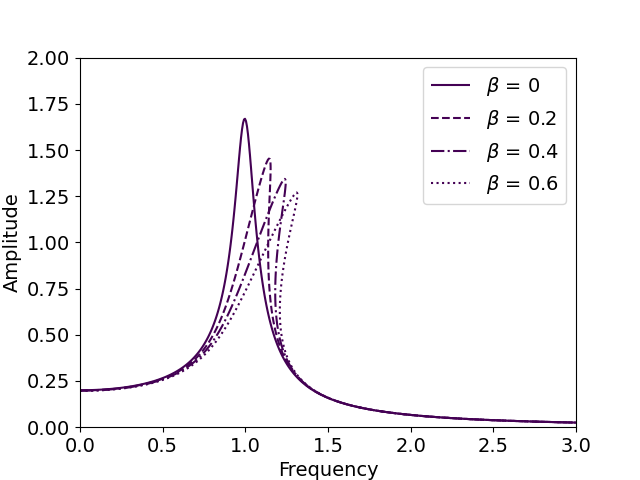
\includegraphics[width=0.5\hsize]{Duffing_freq_betas.png}};
%\node[circle,white,fill=black] at (-2,2){\small (a)};
\node[left,black,fill=white]at (0.5,3.25) {\small (a)};
\end{tikzpicture}
 & 
 \begin{tikzpicture}
\node (image) at (0,0) { 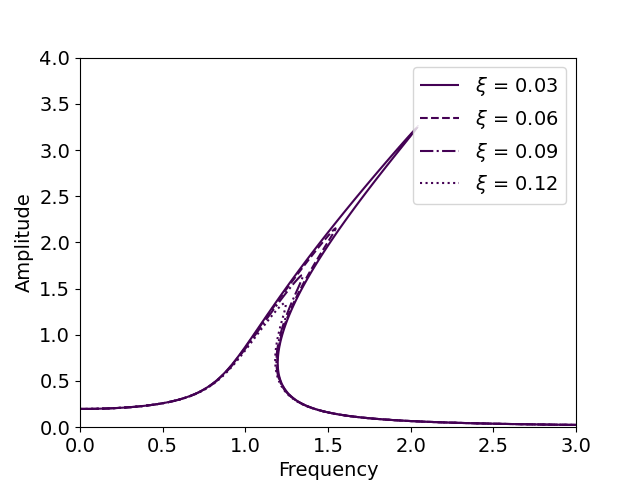
\includegraphics[width=0.5\hsize]{Duffing_freq_Xis.png}};
%\node[circle,white,fill=black] at (-2,2){\small (a)};
\node[left,black,fill=white]at (0.5,3.25) {\small (b)};
\end{tikzpicture}  
\end{tabular}
 \caption{\label{Duffing_frequencies} Resonance curves for (a)  various non-linear stiffnesses with $\chi_0= 0.2$ and $\xi = 0.12$ and (b) various damping coefficients $\chi_0= 0.2$ and $\beta = 0.4$.}
\end{center}
\end{figure}

Being a single potential well oscillator with a hardening stiffness, the pipeline vibrates at the imposed frequency when the amplitude of the applied force is small, as shown in Figure \ref{Duffing_Response}. However, the motion becomes increasingly complex as the amplitude of the applied force increases. Figure \ref{Duffing_Response_chaos} shows that the system is no longer oscillating at the imposed frequency only. Instead, it explores multiple frequencies in a phenomenon known as period doubling bifurcation or 1:2 resonance. This change in the frequency of vibration may be significant as it has a direct consequence on the number of fatigue cycles that the pipeline may experience and on the magnitudes of stresses that it can experience. 
 
 \begin{figure}[H]
\begin{center}
\begin{tabular}{c c}
\begin{tikzpicture}
\node (image) at (0,0) { 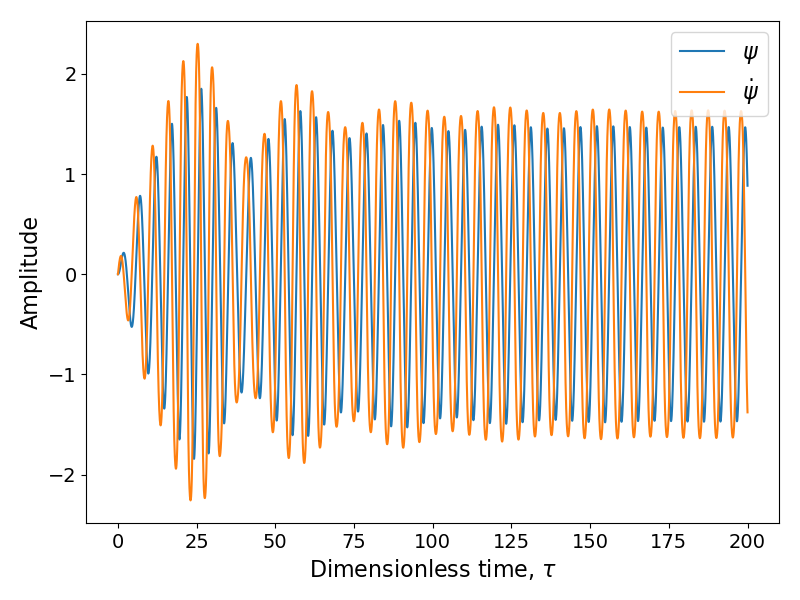
\includegraphics[width=0.5\hsize]{Duffing_TimeSeries.png}};
%\node[circle,white,fill=black] at (-2,2){\small (a)};
\node[left,black,fill=white]at (0.5,3.25) {\small (a)};
\end{tikzpicture}
 & 
 \begin{tikzpicture}
\node (image) at (0,0) { 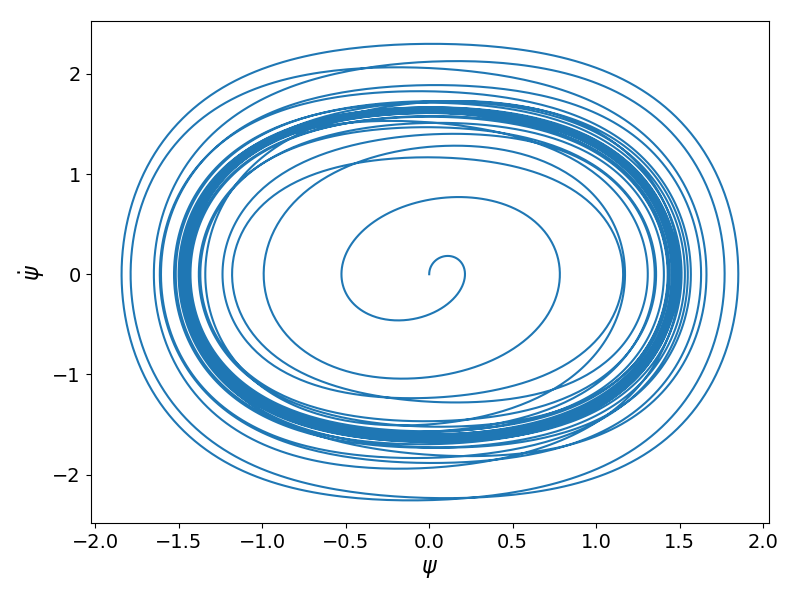
\includegraphics[width=0.5\hsize]{Duffing_PhaseDiag.png}};
%\node[circle,white,fill=black] at (-2,2){\small (a)};
\node[left,black,fill=white]at (0.5,3.25) {\small (b)};
\end{tikzpicture}  
\end{tabular}
 \caption{\label{Duffing_Response} System vibrates smoothly at the imposed frequency when the amplitude of the applied force is small ($\chi_0 = 0.3$, $\xi = 0.06$, $\beta = 0.4$, and $\varpi = 1.2$). }
\end{center}
\end{figure}


 \begin{figure}[H]
\begin{center}
\begin{tabular}{c c}
\begin{tikzpicture}
\node (image) at (0,0) { 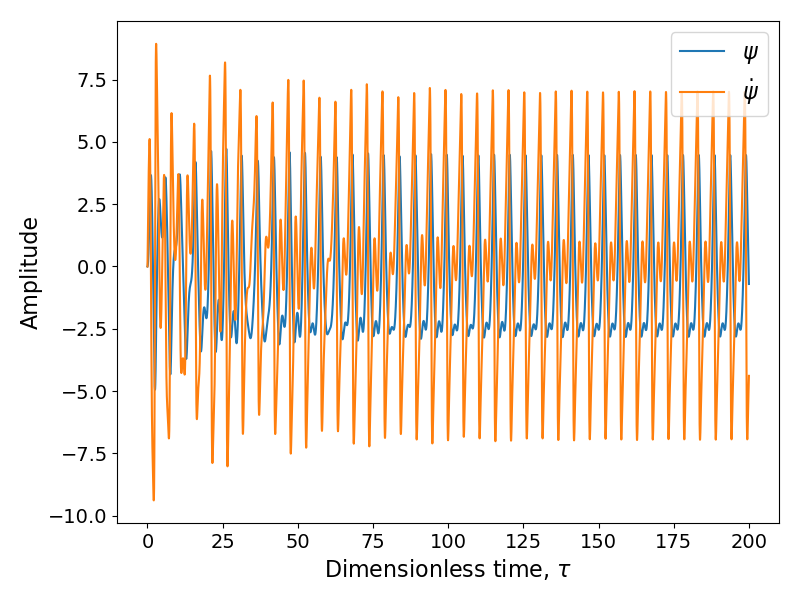
\includegraphics[width=0.5\hsize]{Duffing_TimeSeries_chaos.png}};
%\node[circle,white,fill=black] at (-2,2){\small (a)};
\node[left,black,fill=white]at (0.5,3.25) {\small (a)};
\end{tikzpicture}
 & 
 \begin{tikzpicture}
\node (image) at (0,0) { 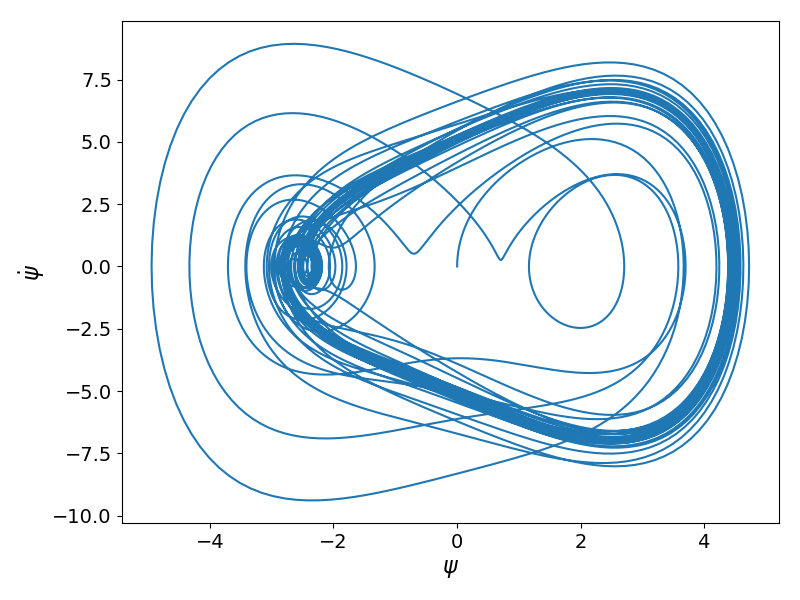
\includegraphics[width=0.5\hsize]{Duffing_PhaseDiag_chaos.png}};
%\node[circle,white,fill=black] at (-2,2){\small (a)};
\node[left,black,fill=white]at (0.5,3.25) {\small (b)};
\end{tikzpicture}  
\end{tabular}
 \caption{\label{Duffing_Response_chaos} System experiences period doubling bifurcations when the amplitude of the applied force is higher ($\chi_0 = 10$, $\xi = 0.06$, $\beta = 0.4$, and $\varpi = 1.2$). }
\end{center}
\end{figure}
 

\section{Conclusions}
In this paper, we investigated the behaviour of free-spanning offshore pipelines (e.g. flowline) that are partially reposing on seabed shoulders and constrained by the seabed or artificial supports (e.g. buckle initiators). We considered the effects of transversal or lateral defections which resulted in non-linear responses that have been overlooked in existing research on pipelines. We opted for closed solutions where the inputs and their influence on the results are unambiguous, which allowed us to investigate the different aspects of pipeline response effectively. In the quasi-static case, the results were generated in the form of pipeline deflection curves reflecting the structural responses under various loading conditions. %These results were compared to field measurement and good agreements have been obtained between the proposed solutions and the field observations, especially when the the sea bed shoulders are flat.  

In the case of vibration, explicit mathematical expressions or semi-analytical procedures were proposed to evaluate the natural frequencies of the pipeline interacting with seawater and the seabed. The particularity of the proposed approach is that it accounts for the effect of large deformation in the pipeline i.e. the current work takes into account mid-plane stretching, which has a strong influence on the static and dynamic responses of the structure. It also considers the effects of distributed transversal and axial forces. 

Based on this study, the following conclusions can be drawn: 
\begin{itemize}
  \item The natural frequencies of the system depend non-linearly on key physical properties including effective mass, pipeline stiffness, and shoulder geometrical and mechanical properties.
  \item Taking the effect of mid-plane stretching into consideration increases the natural frequencies of the system. This is because the effects of the non-linear displacements add up to the axial forces and affect the vibration.  
  \item The natural frequencies of the system decrease when the compressive (resp. tensile) axial force increases (resp. decreases).   
  \item When transversal mid-plane stretching is considered, the differential equations are no longer linear and the superposition principle cannot apply to conduct modal analysis. 
  \item Employing Galerkin's method to solve this problem shows that the frequency of resonance increases with the amplitude of vibration. 
   \item The variation of frequency with respect to amplitude is a function of damping and non-linear stiffness. 
  \item Once the forced oscillation of the pipeline reaches a certain threshold, a period doubling bifurcation occurs, which may influence the fatigue damage.
\end{itemize}

Future work will focus on the significance of mid-plane stretching on the fatigue life of pipelines and cables. Since mid-plane stretching influences the natural frequencies and the deflections, it is expected to influence the distribution of stresses and the number of loading cycles, which can directly impact fatigue damage.    

%\section*{Appendix}
\appendix 
\section{Governing equations based on Hamilton's principle} 
\label{appendix_first}

The governing equations of motion of the pipeline can be derived from the Hamilton's principle as
%%%%%%%%%%%%%%%%%
\begin{equation}\label{Hamilton_pple}
\delta \int_{0}^{\hat{t}}\left ( \mathcal{T} -\Pi + \mathcal{W} \right )\textup{d}\hat{t}=0  % \delta \int_{0}^{\hat{t}}\left ( \mathcal{T} -\Pi + \mathcal{D} - \mathcal{W} \right )\textup{d}t=0
\end{equation}
%%%%%%%%%%%%%%%%%
where $\delta$ represents the variation symbol, $\mathcal{T}$ is the kinetic energy, $\Pi$ is the total potential energy (containing the strain energy of stored in the pipeline and the potential energy due to the interaction of the pipeline with its ground support), and $\mathcal{W}$ is the work done by the external forces during a time interval $\left [ 0,\hat{t} \right ]$. The first variation of the kinetic energy, the potential energy and the virtual work have the following forms
%%%%%%%%%%%%%%%%% $\mathcal{D}$ is the work done by nonconservative force,
\begin{equation}\label{Eq_4_1}
\delta \int_{0}^{\hat{t} } \mathcal{T} \textup{d} \hat{t} = \delta \int_{0}^{\hat{t}}\left \{\frac{1}{2}\int_\Omega \rho \left [\left ( \frac{\partial \hat{u}}{\partial \hat{t}} \right )^2+ \left ( \frac{\partial \hat{v}}{\partial \hat{t}} \right )^2+\left ( \frac{\partial \hat{w}}{\partial \hat{t}} \right )^2 \right ]\textup{d} \Omega \right \}\textup{d}  \hat{t} 
\end{equation}
%%%%
\begin{equation}\label{Eq_4_2} 
\begin{aligned}
 \delta \int_{0}^{\hat{t}}\Pi \textup{d} \hat{t} = \int_{0}^{\hat{t} }  \Biggl\{ \int_{\Omega} \boldsymbol{S}: \delta \boldsymbol{E} d\Omega + \frac{1}{2} \delta \int_{0}^{L_s}\left ( K_v \hat{v}^2  + K_w \hat{w}^2 \right )\textup{d}\hat{x} \Biggr\} \textup{d} \hat{t} 
\end{aligned}
\end{equation}
%%%%
%\begin{equation}\label{Eq_4_3} 
%\begin{aligned}
% & \delta \int_{0}^{\hat{t}} \mathcal{D} \textup{d} \hat{t} = \int_{0}^{\hat{t} }  \frac{1}{2} \delta \int_{-L}^{L_s}\left [ C_v   \left ( \frac{\partial \hat{v}}{\partial \hat{t}} \right )^2 +  C_w  \left ( \frac{\partial \hat{w}}{\partial \hat{t}} \right )^2  \right ]\textup{d}\hat{x} \textup{d} \hat{t} 
%\end{aligned}
%\end{equation}
%%%%
\begin{equation}\label{Eq_4_4}
\delta\int_{0}^{\hat{t}} \mathcal{W}  \textup{d} \hat{t} =\int_{0}^{\hat{t}}\left \{ \int_{-L}^{L_s}\left [q_v(\hat{x},\hat{t}) \delta \hat{v} + q_w(\hat{x},\hat{t}) \delta \hat{w}  \right ] \textup{d}\hat{x} + N_0 (L_s,\hat{t})  \delta \hat{u} \right \}\textup{d} \hat{t} 
\end{equation}
%%%%%%%%%%%%%%%%%
where $\rho$ is the density in the Lagrangian domain $\Omega$, $\hat{u}$ is the axial displacement, $\hat{v}$ is a transversal displacement and $\hat{w}$ is the lateral displacement (here the transversal direction corresponds is the minor direction where small displacements occur as opposed to the lateral direction where larger displacements occur; it can be vertical or horizontal without loss of generality), $\boldsymbol{S}$ is the second Piola-Kirchhoff stress, $\boldsymbol{E}$ is Green-Lagrange strain tensor, which reads $\boldsymbol{E} =  \frac{1}{2} \left(  \nabla_X  \boldsymbol{u}^\flat +  \nabla_X \boldsymbol{u} +   \nabla_X \boldsymbol{u}^\flat \cdot  \nabla_X \boldsymbol{u} \right)$, $\nabla_X$ is the gradient operator in the reference configuration, $\boldsymbol{u} = (\hat{u},\hat{v},\hat{w})^\flat $ is the vector of displacement, $^\flat$ is the transpose operator, $C$ is a viscous damping coefficient in the proper direction, $K$ is the soil stiffness in the proper direction, $q(\hat{x},\hat{t})$ is the hydrodynamic and/or gravity load in the proper direction denoted by the subscripts $\hat{v}$ or $\hat{w}$, and $N_0 (L_s,\hat{t}) $ is an axial force applied at the end of the pipeline. The beam is assumed to occupy the interval $[-L,L_s]$ such that $[-L,0]$ is the area of free span and $[0,L_s]$ is the area of pipeline-seabed interaction (see Figure \ref{ISL_system}). 

 The strain $\boldsymbol{E}$ is decomposed into a linear component $\boldsymbol{e}^{l} = \frac{1}{2} \left(\nabla_X\boldsymbol{u}^\flat +  \nabla_X\boldsymbol{u} \right) $ and a non-linear component  $\boldsymbol{e}^{nl} = \frac{1}{2} \left( \nabla_X\boldsymbol{u} ^\flat \cdot  \nabla_X\boldsymbol{u} \right)$. The stress $\boldsymbol{S}$ can be linearised to the first order as $\boldsymbol{S} = \mathbb{C}:\boldsymbol{E}$, where $\mathbb{C}$ is the fourth order elasticity tensor. The only significant term in the Green-Lagrange strain tensor is $E_{11} = \hat{u}_{,\hat{x}} + \frac{1}{2} \left( \hat{u}_{,\hat{x}}^2 + \hat{v}_{,\hat{x}}^2 + \hat{w}_{,\hat{x}}^2 \right)$ such that $e^{l} =  \hat{u}_{,\hat{x}}$ and  $e^{nl} =  \frac{1}{2} \left( \hat{u}_{,\hat{x}}^2 + \hat{v}_{,\hat{x}}^2 + \hat{w}_{,\hat{x}}^2 \right)$. Therefore, the potential energy of the pipeline is
 
  \begin{equation}\label{PVWMoreSimplified}
  \begin{array}{l } 
\displaystyle \int_{\Omega} \left(\boldsymbol{E}: \mathbb{C}:  \delta \boldsymbol{e}^{l}  + \boldsymbol{S}: \delta \boldsymbol{e}^{nl}  \right)  d\Omega  =  
\displaystyle E \int_{-L}^{L_s} \int_{A} E_{11}\left(\delta e^{l} + \delta e^{nl} \right) dA \textup{d}\hat{x} \\
  \end{array}  
 \end{equation}
 Based on the Kirchhoff--Love hypotheses requiring that the surface normals to the neutral line remain normal after deformation and that any changes in the thickness/diameter of the pipe are negligible.
 \begin{equation}\label{Displacement}
\begin{array}{l }
\hat{u} = \tilde{u} (\hat{x}) - y \frac{\partial \hat{v}}{\partial \hat{x}} - z \frac{\partial \hat{w}}{\partial \hat{x}}; \quad \hat{v} = \hat{v} (\hat{x}) \text{ and } \hat{w} = \hat{w} (\hat{x}) \\
  \end{array}  
\end{equation}
Hence, using the definition of curvature $\kappa_y = -\frac{\partial^2 \hat{w}}{\partial \hat{x}^2}$ and $\kappa_z = -\frac{\partial^2 \hat{v}}{\partial \hat{x}^2}$ and neglecting the quadratic term $\tilde{u}_{,\hat{x}} ^2$ compared to $\hat{v}_{,\hat{x}}^2$ and $\hat{w}_{,\hat{x}}^2$ , the strains can be expressed as 
 \begin{equation}\label{Deformation}
\begin{array}{l }
e^{l}  =   \tilde{u}_{,\hat{x}} + y \kappa_z + z \kappa_y  \text{ and } e^{nl} \approx  \frac{1}{2} \left( \hat{v}_{,\hat{x}}^2 + \hat{w}_{,\hat{x}}^2 \right)  \\
  \end{array}  
\end{equation}
Substituting Equation (\ref{Deformation}) into Equation (\ref{PVWMoreSimplified}) and using the notation $\epsilon= \tilde{u}_{,\hat{x}} $ gives
  \begin{equation}\label{PVWMoreSimplified_bis}
  \begin{array}{l l} 
\displaystyle E \int_{-L}^{L_s} \int_{A} E_{11}\left(\delta e^{l} + \delta e^{nl} \right) dA \textup{d} \hat{x}  &  \displaystyle = \int_{-L}^{L_s} \left( N \delta \left[\epsilon + \frac{1}{2} \left(\hat{v}_{,\hat{x}}^2 + \hat{w}_{,\hat{x}}^2 \right) \right]+ M_y \delta \kappa_z + M_z \delta \kappa_y \right) \textup{d} \hat{x}\\
& \displaystyle = \int_{-L}^{L_s} \left( N \left[ \delta \epsilon + \hat{v}_{,\hat{x}}  \delta \hat{v}_{,\hat{x}}  + \hat{w}_{,\hat{x}}  \delta \hat{w}_{,\hat{x}}   \right]+ M_y \delta \kappa_z + M_z \delta \kappa_y \right) \textup{d}\hat{x}
  \end{array}  
 \end{equation}
 where the generalised forces are
 
  \begin{equation}\label{generalised_forces}
\begin{array}{l }
\displaystyle  N = E\int_{A}  \left(\epsilon + e^{nl} + y \kappa_z + z \kappa_y \right) dA = E \left( A (\epsilon + e^{nl} )  + S_y \kappa_z + S_z \kappa_y \right) = E A (\epsilon + e^{nl} )   \\ 
\displaystyle M_y =E \int_{A}   \left(\epsilon + e^{nl} + y \kappa_z + z \kappa_y \right) y   dA = E \left(S_y (\epsilon + e^{nl} ) + I_{yy} \kappa_z + I_{yz} \kappa_y \right) = EI \kappa_z  \\ 
\displaystyle M_z = E\int_{A}   \left(\epsilon + e^{nl} + y \kappa_z + z \kappa_y \right) z  dA =  E \left(S_z (\epsilon + e^{nl} ) + I_{yz} \kappa_z + I_{zz} \kappa_y \right) = EI \kappa_y \\ 
  \end{array}  
\end{equation}
where $A =\displaystyle \int_{A} dA$  , $S_y \displaystyle \int_{A} y dA$,  $S_z = \displaystyle \int_{A} z dA$ ,$I_{yy} =\displaystyle \int_{A} y^2 dA$, $I_{yz} =\displaystyle \int_{A} yz dA$  and $I_{zz} = \displaystyle \int_{A} z^2dA$ are geometrical constants that depend on the shape of the pipeline only. When the cross section of the pipeline is symmetric (which is the case for tubular shapes), $S_y= S_z = 0$ and $I_{yz} = 0$. The non-zero constants $A$, $I_{yy}$ and $I_{zz}$ are the area and the bending moments of inertia around the y- and z-axes, respectively. Because of symmetry, $I_{yy}=I_{zz} = I$, as seen in Equation (\ref{generalised_forces}). Integrating Equation (\ref{PVWMoreSimplified_bis}) by parts shows that

  \begin{equation}\label{PVWMoreSimplified_sec}
  \begin{array}{l} 
\displaystyle \int_{-L}^{L_s} \left( N \left[ \delta \epsilon + \hat{v}_{,\hat{x}}  \delta \hat{v}_{,\hat{x}}  + \hat{w}_{,\hat{x}}  \delta \hat{w}_{,\hat{x}}   \right]+ M_y \delta \kappa_z + M_z \delta \kappa_y \right) \textup{d}\hat{x} \\
\displaystyle  = - \int_{-L}^{L_s} \left( N_{,\hat{x}} \delta  \tilde{u} + (N \hat{v}_{,\hat{x}})_{,\hat{x}}  \delta \hat{v}  + (N \hat{w}_{,\hat{x}})_{,\hat{x}}  \delta \hat{w}   + M_{y,\hat{x}\hat{x}} \delta \hat{v} + M_{z,\hat{x}\hat{x}} \delta \hat{w} \right) \textup{d}\hat{x} \\
\displaystyle  + \oint_{-L}^{L_s} \left( N n_x \delta  \tilde{u} + N \hat{v}_{,\hat{x}} n_x  \delta \hat{v}  + N \hat{w}_{,\hat{x}} n_x  \delta \hat{w}   + M_y n_x \delta \hat{v}_{,\hat{x}} + M_z n_x \delta \hat{w}_{,\hat{x}}  + M_{y,\hat{x}} n_x \delta \hat{v} + M_{z,\hat{x}} n_x \delta \hat{w}\right) \textup{d}\hat{x}
  \end{array}   
 \end{equation}
 
Similarly, it can be seen from Equation \ref{Eq_4_1} that 
\begin{equation}\label{kineticEnergy}
  \begin{array}{l } 
\displaystyle 
\delta \int_{0}^{\hat{t}} \mathcal{T}  d \hat{t}=  \int_{0}^{\hat{t}} A \rho \int_{-L}^{L_s} \left( \frac{\partial \hat{u}}{\partial \hat{t}} \delta \left(\frac{\partial \hat{u}}{\partial \hat{t}} \right)+  \frac{\partial \hat{v}}{\partial \hat{t}} \delta \left(\frac{\partial \hat{v}}{\partial \hat{t}} \right) +  \frac{\partial \hat{w}}{\partial \hat{t}} \delta \left(\frac{\partial \hat{w}}{\partial \hat{t}}  \right) \right)\textup{d} \hat{x}  d \hat{t}
  \end{array}  
\end{equation}
Integration Equation {\ref{kineticEnergy}} by parts and assuming that the variations vanish at the two ends of the time intervals results in 
\begin{equation}\label{kineticEnergy_2}
  \begin{array}{l } 
\displaystyle 
\delta \int_{0}^{\hat{t}} \mathcal{T}  d \hat{t}=  - m_e \int_{0}^{\hat{t}}  \int_{-L}^{L_s} \left( \frac{\partial^2 \hat{u}}{\partial \hat{t}^2} \delta \hat{u} +  \frac{\partial^2 \hat{v}}{\partial \hat{t}^2} \delta \hat{v} +  \frac{\partial^2 \hat{w}}{\partial \hat{t}^2} \delta \hat{w} \right) \textup{d} \hat{x}  d \hat{t}
  \end{array}  
\end{equation}
Replacing the potential and kinetic energy expressions (\ref{PVWMoreSimplified_sec}) and (\ref{kineticEnergy_2}) in Equation (\ref{Hamilton_pple}) shows that

\begin{equation}\label{Hamilton_pple_2}
  \begin{array}{l } 
\displaystyle - \int_{0}^{\hat{t}}\left \{ m_e \int_{-L}^{L_s} \left( \frac{\partial^2 \hat{u}}{\partial \hat{t}^2} \delta \hat{u} +  \frac{\partial^2\hat{v}}{\partial \hat{t}^2} \delta \hat{v} +  \frac{\partial^2 \hat{w}}{\partial \hat{t}^2} \delta \hat{w} \right)\textup{d} \hat{x}   \right .\\
\displaystyle \left.  + \int_{-L}^{L_s} \left( N_{,\hat{x}} \delta  \tilde{u} + (N \hat{v}_{,\hat{x}})_{,\hat{x}}  \delta \hat{v}  + (N \hat{w}_{,\hat{x}})_{,\hat{x}}  \delta \hat{w}   + M_{y,\hat{x}\hat{x}} \delta \hat{v} + M_{z,\hat{x}\hat{x}} \delta \hat{w} \right) \textup{d} \hat{x} \right .\\
\displaystyle \left.  - \oint_{-L}^{L_s} \left( N n_x \delta  \tilde{u} + N \hat{v}_{,\hat{x}} n_x  \delta \hat{v}  + N \hat{w}_{,\hat{x}} n_x  \delta \hat{w}   + M_y n_x \delta \hat{v}_{,\hat{x}} + M_z n_x \delta \hat{w}_{,\hat{x}}  + M_{y,\hat{x}} n_x \delta \hat{v} + M_{z,\hat{x}} n_x \delta \hat{w}\right) \textup{d} \hat{x} \right .\\
\displaystyle \left.- \int_{0}^{L_s}\left ( K_v \hat{v} \delta \hat{v}   + K_w \hat{w} \delta \hat{w}  \right )\textup{d}\hat{x} + \int_{-L}^{L_s}\left [q_v( x,\hat{t}) \delta \hat{v} + q_w( x,\hat{t}) \delta \hat{w}  \right ] \textup{d}\hat{x} + N_0 (L_s, \hat{t}) \delta \hat{u} \right \}\textup{d}\hat{t}=0  % \delta \int_{0}^{\hat{t}}\left ( \mathcal{T} -\Pi + \mathcal{D} - \mathcal{W} \right )\textup{d}t=0
  \end{array}  
\end{equation}
 
Rearranging the terms in the internal longitudinal integral 
 
  \begin{equation}\label{system_differential_equation_0}
  \begin{array}{l } 
  \displaystyle  m_e  \frac{\partial^2 \hat{u}}{\partial \hat{t}^2} =  N_{,\hat{x}} \\ 
  \displaystyle m_e  \frac{\partial^2 \hat{v}}{\partial \hat{t}^2} + K_v \mathcal{I}_{[0,L_s]} \hat{v} = (N \hat{v}_{,\hat{x}})_{,\hat{x}}  + M_{y,\hat{x}\hat{x}}  + q_v(\hat{x},\hat{t}) \\ 
  \displaystyle m_e  \frac{\partial^2 \hat{w}}{\partial \hat{t}^2} + K_w \mathcal{I}_{[0,L_s]} \hat{w} = (N \hat{w}_{,\hat{x}})_{,\hat{x}}  + M_{z,\hat{x}\hat{x}} + q_w(\hat{x},\hat{t}) \\ 
  \end{array}  
\end{equation}
The closed integral can be used to deduce the boundary conditions such as $N_0 (L_s,\hat{t})  = N(L_s,\hat{t}) n_x$ (these conditions are omitted in this appendix). Given the definition in Equation (\ref{generalised_forces}) stating that $N = E A (\epsilon + e^{nl} ) = E A(\tilde{u}_{,\hat{x}} + \frac{1}{2} \left( \hat{v}_{,\hat{x}}^2 + \hat{w}_{,\hat{x}}^2 \right))$, the first differential equation in the system (\ref{system_differential_equation_0}) can be expressed as

  \begin{equation}\label{first_differential_equation}
  \begin{array}{l } 
  \displaystyle  m_e  \frac{\partial^2 \hat{u}}{\partial \hat{t}^2}  - E A \tilde{u}_{,\hat{x}\hat{x}}=  \frac{E A }{2} \left( \hat{v}_{,\hat{x}}^2 + \hat{w}_{,\hat{x}}^2 \right)_{,\hat{x}} \\  
  \end{array}  
\end{equation}

Since the beam is slender (small radius of gyration $r = \sqrt{I/A}$), the natural transversal and lateral frequencies are much smaller than the natural axial frequency and the inertial term $m_e \frac{\partial^2 \hat{u}}{\partial \hat{t}^2}$ is negligible. Therefore, Equation (\ref{first_differential_equation}) shows that the axial deformation can be related to the transversal and lateral deformations: $\tilde{u}_{,\hat{x}\hat{x}}=  - \frac{1}{2} \left( \hat{v}_{,\hat{x}}^2 + \hat{w}_{,\hat{x}}^2 \right)_{,\hat{x}} $. Integrating this expression shows that 

  \begin{equation}\label{Integrating_axial_Displ_0}
  \begin{array}{l } 
  \displaystyle  \tilde{u} = -  \frac{1}{2} \int_{-L}^{\hat{x}} \left( \hat{v}_{,\hat{x}}^2 + \hat{w}_{,\hat{x}}^2 \right) \textup{d} \hat{x} + c(\hat{t}) \hat{x} + c_1(\hat{t}) \\  
  \end{array}  
\end{equation}
where $c(\hat{t})$ and $c_1(\hat{t})$ are constants of integration that are independent of space but dependent on time. If the pipeline is fixed axially at $\hat{x}=-L$, then $c(\hat{t}) L =  c_1(\hat{t})$ and $  \displaystyle\tilde{u} = -  \frac{1}{2} \int_{-L}^{\hat{x}} \left( \hat{v}_{,\hat{x}}^2 + \hat{w}_{,\hat{x}}^2 \right) \textup{d} \hat{x} + c(\hat{t}) (\hat{x} + L)$. If an axial force $N(\hat{t})$ is applied to the pipeline causing the axial deformation it can be verified that $  \displaystyle \tilde{u} (L_s) +  \frac{1}{2} \int_{-L}^{L_s} \left( \hat{v}_{,\hat{x}}^2 + \hat{w}_{,\hat{x}}^2 \right) \textup{d} \hat{x} = c(\hat{t}) (L_s+L)$ and $c(\hat{t}) =\frac{N(\hat{t})}{EA}$. Hence the axial force can be written as 

  \begin{equation}\label{Integrating_axial_Displ_Ls}
  \begin{array}{l } 
  \displaystyle N  = \frac{EA}{L+Ls}\left( \tilde{u} (L_s) +  \frac{1}{2} \int_{-L}^{L_s} \left( \hat{v}_{,\hat{x}}^2 + \hat{w}_{,\hat{x}}^2 \right) \textup{d} \hat{x} \right)= N_0 + \frac{EA}{2(L+L_s)} \int_{-L}^{L_s} \left( \hat{v}_{,\hat{x}}^2 + \hat{w}_{,\hat{x}}^2 \right) \textup{d} \hat{x}   
  \end{array}  
\end{equation}
where $N_0 = \frac{EA \tilde{u} (L_s)}{L+Ls} $.  Substituting Equation (\ref{Integrating_axial_Displ_Ls}) into Equation (\ref{system_differential_equation_0})
  \begin{equation}\label{system_differential_equation}
  \begin{array}{l } 
%  \displaystyle  m_e  \frac{\partial^2 \hat{u}}{\partial \hat{t}^2} =  N_{,\hat{x}} \\ 
  \displaystyle m_e  \frac{\partial^2 \hat{v}}{\partial \hat{t}^2} + EI \frac{\partial^4 \hat{v}}{\partial \hat{x}^4} - N_0 \frac{\partial^2 \hat{v}}{\partial \hat{x}^2} + K_v \mathcal{I}_{[0,L_s]} \hat{v} =\frac{EA}{2(L+L_s)} \frac{\partial^2 \hat{v}}{\partial \hat{x}^2}  \int_{-L}^{L_s} \left( \hat{v}_{,\hat{x}}^2 + \hat{w}_{,\hat{x}}^2 \right) \textup{d} \hat{x}  + q_v(\hat{x},\hat{t}) \\ 
    \displaystyle m_e  \frac{\partial^2 \hat{w}}{\partial \hat{t}^2} + EI \frac{\partial^4 \hat{w}}{\partial \hat{x}^4} - N_0 \frac{\partial^2 \hat{w}}{\partial \hat{x}^2} + K_w \mathcal{I}_{[0,L_s]} \hat{w} =\frac{EA}{2(L+L_s)} \frac{\partial^2 \hat{w}}{\partial \hat{x}^2}  \int_{-L}^{L_s} \left( \hat{v}_{,\hat{x}}^2 + \hat{w}_{,\hat{x}}^2 \right) \textup{d} \hat{x}  + q_w(\hat{x},\hat{t})  
  \end{array}  
\end{equation} 
It can be seen that the differential equations in terms of $\hat{v}$ and $\hat{w}$ are identical --- the governing equations are the same for in-line (horizontal) and cross-flow (vertical) vibration and they are treated in a similar manner. 
 
 
\section*{Acknowledgements} The authors would like to acknowledge the valuable comments on an early draft of this paper with Ralf Peek. This research was supported by the Australian Research Council Industrial Transformation Research Hubs scheme (Grant No. IH200100009) through the project Transforming energy Infrastructure through Digital Engineering (TIDE, http://TIDE.edu.au).


%\section{References}
\bibliographystyle{APA}
%\bibliographystyle{unsrt}
\bibliography{References}

    
\end{document} 

